% =====================================================================
%  Paper 4 — RetinAI: from hand-crafted features to vision transformers. IEEE journal layout (IEEEtran).
%  Build:  .venv/bin/python scripts/paper4_figures.py   (writes figs4/: figures, tab_*.tex, numbers4.tex; regenerates
%          the figs3/ tables and figures this file inputs)
%          tectonic -X compile paper4_journey.tex
%  Every number in this file is a macro from figs4/numbers4.tex or a cell of a generated table; none is typed here.
%  Items in \FILL{...} must be completed by the authors before submission.
% =====================================================================
\documentclass[journal]{IEEEtran}
\usepackage{graphicx,booktabs,amsmath,amssymb,xcolor,url,array}
\graphicspath{{figs4/}{figs3/}{figs2/}}
\newcommand{\FILL}[1]{\textcolor{red}{\textbf{[FILL: #1]}}}
\IEEEoverridecommandlockouts
\usepackage{iftex}\ifXeTeX\usepackage{fontspec}\setmainfont{texgyretermes}[Extension=.otf,UprightFont=*-regular,BoldFont=*-bold,ItalicFont=*-italic,BoldItalicFont=*-bolditalic]\fi
\raggedbottom
% generated by scripts/paper4_figures.py (includes every macro of scripts/paper3_figures.py); do not edit
\newcommand{\selArm}{B}
\newcommand{\BcvQ}{0.825}
\newcommand{\BcvQci}{[0.737, 0.911]}
\newcommand{\BdevQ}{0.756}
\newcommand{\BdevQci}{[0.679, 0.821]}
\newcommand{\BlosoQ}{0.834}
\newcommand{\nArms}{9}
\newcommand{\nTrained}{7}
\newcommand{\poolImages}{6{,}700}
\newcommand{\poolInfants}{1{,}528}
\newcommand{\poolSources}{3}
\newcommand{\dupExcl}{14}
\newcommand{\cvScored}{6{,}686}
\newcommand{\devImages}{663}
\newcommand{\devEyes}{230}
\newcommand{\devInfants}{116}
\newcommand{\lockedImages}{661}
\newcommand{\lockedEyes}{230}
\newcommand{\nReps}{2{,}000}
\newcommand{\bootSeed}{42}
\newcommand{\cvLists}{2}
\newcommand{\devLists}{10}
\newcommand{\seedA}{42}
\newcommand{\seedB}{1337}
\newcommand{\marginCV}{0.010}
\newcommand{\marginLOSO}{0.010}
\newcommand{\nAmend}{5}
\newcommand{\lastAmendDate}{2026-10-31}
\newcommand{\protoCommit}{ac33f29}
\newcommand{\protoDate}{2026-10-20}
\newcommand{\nArch}{11}
\newcommand{\nArmsAll}{20}
\newcommand{\transArms}{F}
\newcommand{\nPairs}{12}
\newcommand{\nRuns}{10}
\newcommand{\shortcutAUC}{0.911}
\newcommand{\lockedOpened}{2026-08-18}
\newcommand{\nSevereFrom}{3}
\newcommand{\gpu}{Tesla T4}
\newcommand{\mateN}{3{,}141}
\newcommand{\mateMatched}{2{,}964}
\newcommand{\mateUnmatched}{177}
\newcommand{\mateSrcRopvl}{1{,}438}
\newcommand{\mateSrcMultiview}{896}
\newcommand{\mateSrcShenzhen}{630}
\newcommand{\mateDevTrain}{390}
\newcommand{\mateLockedTrain}{331}
\newcommand{\matePoolTrain}{1{,}647}
\newcommand{\mateTrain}{2{,}512}
\newcommand{\mateVal}{314}
\newcommand{\mateTest}{315}
\newcommand{\mateMLTest}{629}
\newcommand{\mateLeakTest}{73\%}
\newcommand{\mateLeakVal}{73\%}
\newcommand{\mateLeakMV}{99\%}
\newcommand{\mateMLFeat}{428}
\newcommand{\mateMLBest}{SVM (RBF)}
\newcommand{\mateMLAcc}{0.585}
\newcommand{\mateMLQ}{0.547}
\newcommand{\mateCNNBest}{resnest50d}
\newcommand{\mateCNNAcc}{0.835}
\newcommand{\mateCNNQ}{0.898}
\newcommand{\mateCNNEnsAcc}{0.825}
\newcommand{\mateCNNDiverged}{convnext\_tiny}
\newcommand{\mateCNNDivergedAcc}{0.530}
\newcommand{\mateFMlo}{0.787}
\newcommand{\mateFMhi}{0.832}
\newcommand{\mateFMmean}{0.814}
\newcommand{\mateFMsd}{0.023}
\newcommand{\mateFMtrainable}{6.30}
\newcommand{\mateFMtotal}{309.7}
\newcommand{\mateFMbaseAcc}{0.825}
\newcommand{\mateFMbaseTrainable}{2.37}
\newcommand{\mateFMcomboAcc}{0.651}
\newcommand{\mateEnsAcc}{0.844}
\newcommand{\mateEnsQ}{0.900}
\newcommand{\mateBestAcc}{0.860}
\newcommand{\mateBestQ}{0.908}
\newcommand{\mateBestAUC}{0.972}
\newcommand{\mateBestN}{7}
\newcommand{\mateBestAccci}{[0.820, 0.896]}
\newcommand{\mateCIkind}{infant-clustered bootstrap}
\newcommand{\mateHalfWidth}{4}
\newcommand{\mateCommit}{424ad77}
\newcommand{\nMateSeries}{33}
\newcommand{\mateDate}{2026-11-07}
\newcommand{\acqImages}{13{,}037}
\newcommand{\acqSources}{11}
\newcommand{\acqExcluded}{2{,}610}
\newcommand{\stageLabelled}{10{,}427}
\newcommand{\stageInfants}{2{,}015}
\newcommand{\sixElig}{8{,}024}
\newcommand{\sixInfants}{1{,}760}
\newcommand{\exclOther}{1{,}295}
\newcommand{\exclTreated}{1{,}063}
\newcommand{\exclStageZero}{45}
\newcommand{\exclSix}{2{,}403}
\newcommand{\trainEligible}{3{,}112}
\newcommand{\vfourTrain}{3{,}083}
\newcommand{\poolValOnly}{3{,}588}
\newcommand{\capNormal}{2}
\newcommand{\capOther}{20}
\newcommand{\rawMultiview}{1{,}324}
\newcommand{\rawMultiviewInf}{232}
\newcommand{\rawOstrava}{6{,}004}
\newcommand{\rawOstravaInf}{187}
\newcommand{\rawRopvl}{2{,}020}
\newcommand{\rawRopvlInf}{1{,}116}
\newcommand{\rawShenzhen}{1{,}079}
\newcommand{\rawShenzhenInf}{480}
\newcommand{\poolOstrava}{4{,}285}
\newcommand{\poolOstravaInf}{148}
\newcommand{\perInfantOstrava}{29.0}
\newcommand{\poolRopvl}{1{,}675}
\newcommand{\poolRopvlInf}{983}
\newcommand{\perInfantRopvl}{1.7}
\newcommand{\poolShenzhen}{740}
\newcommand{\poolShenzhenInf}{397}
\newcommand{\perInfantShenzhen}{1.9}
\newcommand{\siteDecodable}{0.997}
\newcommand{\metaFloorCV}{0.187}
\newcommand{\metaFloorDev}{0.062}
\newcommand{\dupExact}{0}
\newcommand{\dupNear}{0}
\newcommand{\humanInterKappa}{0.24}
\newcommand{\humanIntraKappa}{0.56}
\newcommand{\humanDisagree}{40\%}
\newcommand{\vTwoKappaU}{0.655}
\newcommand{\BkappaU}{0.637}
\newcommand{\BdevKappaU}{0.527}
\newcommand{\vOneAcc}{0.733}
\newcommand{\vOneFone}{0.706}
\newcommand{\sweepAUC}{0.927}
\newcommand{\sweepValAUC}{0.842}
\newcommand{\vTwoCvQsix}{0.761}
\newcommand{\vTwoCvAcc}{0.786}
\newcommand{\vTwoLockedImgQ}{0.473}
\newcommand{\vTwoLockedEyeQ}{0.813}
\newcommand{\vTwoLockedEyeAcc}{0.646}
\newcommand{\vTwoGapMin}{0.32}
\newcommand{\vTwoGapMax}{0.34}
\newcommand{\sweepSelAUC}{0.964}
\newcommand{\sweepArchs}{5}
\newcommand{\mateMLReportAcc}{0.568}
\newcommand{\BkappaUpooled}{0.635}
\newcommand{\BdevKappaUpooled}{0.524}
\newcommand{\BthrPct}{98.94\%}
\newcommand{\BcvSens}{0.900}
\newcommand{\BcvSpec}{0.996}
\newcommand{\BdevSens}{0.656}
\newcommand{\BdevSpec}{1.000}
\newcommand{\BdevSevereSens}{0.927}
\newcommand{\BdevECE}{0.157}
\newcommand{\BdevRecNormal}{0.948}
\newcommand{\BcvRecNormal}{0.909}
\newcommand{\BdevRecStageOne}{0.510}
\newcommand{\BcvRecStageOne}{0.583}
\newcommand{\BdevRecStageTwo}{0.546}
\newcommand{\BcvRecStageTwo}{0.561}
\newcommand{\BdevRecStageThree}{0.566}
\newcommand{\BcvRecStageThree}{0.722}
\newcommand{\BdevRecStageFourFive}{0.580}
\newcommand{\BcvRecStageFourFive}{0.882}
\newcommand{\BdevRecArop}{0.700}
\newcommand{\BcvRecArop}{0.389}
\newcommand{\BdevAcc}{0.630}
\newcommand{\BdevMF}{0.566}
\newcommand{\BdevAUC}{0.937}
\newcommand{\BcvAcc}{0.766}
\newcommand{\BcvAUC}{0.979}
\newcommand{\BfoldMinutes}{33}
\newcommand{\nGenerations}{4}
\newcommand{\cvDiffAC}{−0.022}
\newcommand{\cvDiffACci}{[$-$0.052, +0.008]}
\newcommand{\cvDiffAB}{−0.031}
\newcommand{\cvDiffABci}{[$-$0.077, +0.015]}
\newcommand{\cvDiffBC}{+0.009}
\newcommand{\cvDiffBCci}{[$-$0.018, +0.027]}
\newcommand{\cvDiffEC}{+0.005}
\newcommand{\cvDiffECci}{[$-$0.007, +0.019]}
\newcommand{\cvDiffEA}{+0.026}
\newcommand{\cvDiffEAci}{[+0.008, +0.046]}
\newcommand{\cvDiffDA}{+0.002}
\newcommand{\cvDiffDAci}{[$-$0.057, +0.046]}
\newcommand{\cvDiffDB}{−0.029}
\newcommand{\cvDiffDBci}{[$-$0.051, +0.003]}
\newcommand{\cvDiffFB}{−0.014}
\newcommand{\cvDiffFBci}{[$-$0.035, +0.008]}
\newcommand{\cvDiffGB}{−0.011}
\newcommand{\cvDiffGBci}{[$-$0.036, +0.012]}
\newcommand{\cvDiffHB}{−0.013}
\newcommand{\cvDiffHBci}{[$-$0.031, +0.009]}
\newcommand{\cvDiffIB}{−0.004}
\newcommand{\cvDiffIBci}{[$-$0.015, +0.007]}
\newcommand{\cvDiffIH}{+0.009}
\newcommand{\cvDiffIHci}{[$-$0.007, +0.020]}
\newcommand{\devDiffAC}{+0.014}
\newcommand{\devDiffACci}{[$-$0.012, +0.048]}
\newcommand{\devDiffAB}{+0.019}
\newcommand{\devDiffABci}{[+0.000, +0.041]}
\newcommand{\devDiffBC}{−0.004}
\newcommand{\devDiffBCci}{[$-$0.038, +0.030]}
\newcommand{\devDiffEC}{+0.010}
\newcommand{\devDiffECci}{[$-$0.012, +0.040]}
\newcommand{\devDiffEA}{−0.004}
\newcommand{\devDiffEAci}{[$-$0.020, +0.008]}
\newcommand{\devDiffDA}{−0.028}
\newcommand{\devDiffDAci}{[$-$0.048, $-$0.011]}
\newcommand{\devDiffDB}{−0.009}
\newcommand{\devDiffDBci}{[$-$0.019, +0.001]}
\newcommand{\devDiffFB}{−0.012}
\newcommand{\devDiffFBci}{[$-$0.022, $-$0.002]}
\newcommand{\devDiffGB}{+0.012}
\newcommand{\devDiffGBci}{[$-$0.006, +0.032]}
\newcommand{\devDiffHB}{−0.006}
\newcommand{\devDiffHBci}{[$-$0.015, +0.003]}
\newcommand{\devDiffIB}{+0.020}
\newcommand{\devDiffIBci}{[+0.003, +0.041]}
\newcommand{\devDiffIH}{+0.026}
\newcommand{\devDiffIHci}{[+0.006, +0.046]}
\newcommand{\BostravaQ}{0.701}
\newcommand{\BropvlQ}{0.930}
\newcommand{\BshenzhenQ}{0.967}
\newcommand{\DostravaQ}{0.846}
\newcommand{\DropvlQ}{0.925}
\newcommand{\DshenzhenQ}{0.967}
\newcommand{\CostravaQ}{0.775}
\newcommand{\CropvlQ}{0.921}
\newcommand{\CshenzhenQ}{0.967}
\newcommand{\cvQAsA}{0.797}
\newcommand{\devQAsA}{0.772}
\newcommand{\cvQAsB}{0.791}
\newcommand{\devQAsB}{0.776}
\newcommand{\cvQBsA}{0.835}
\newcommand{\devQBsA}{0.754}
\newcommand{\cvQBsB}{0.815}
\newcommand{\devQBsB}{0.757}
\newcommand{\cvQCsA}{0.819}
\newcommand{\devQCsA}{0.756}
\newcommand{\cvQCsB}{0.813}
\newcommand{\devQCsB}{0.764}
\newcommand{\mdd}{0.08}
\newcommand{\eqCvWithin}{12}
\newcommand{\eqCvZero}{11}
\newcommand{\eqCvTotal}{12}
\newcommand{\eqDevWithin}{12}
\newcommand{\eqDevZero}{7}
\newcommand{\eqDevTotal}{12}
\newcommand{\BcvQsix}{0.779}
\newcommand{\BostravaQci}{[0.490, 0.776]}
\newcommand{\BostravaQr}{0.701}
\newcommand{\BropvlQci}{[0.915, 0.943]}
\newcommand{\BropvlQr}{0.930}
\newcommand{\BshenzhenQci}{[0.958, 0.976]}
\newcommand{\BshenzhenQr}{0.967}
\newcommand{\CostravaQci}{[0.522, 0.876]}
\newcommand{\CostravaQr}{0.775}
\newcommand{\CropvlQci}{[0.902, 0.936]}
\newcommand{\CropvlQr}{0.921}
\newcommand{\CshenzhenQci}{[0.957, 0.975]}
\newcommand{\CshenzhenQr}{0.967}
\newcommand{\DostravaQci}{[0.692, 0.917]}
\newcommand{\DostravaQr}{0.846}
\newcommand{\DropvlQci}{[0.909, 0.939]}
\newcommand{\DropvlQr}{0.925}
\newcommand{\DshenzhenQci}{[0.954, 0.976]}
\newcommand{\DshenzhenQr}{0.967}
\newcommand{\devPhotosPerEyeMedian}{3}
\newcommand{\devPhotosPerEyeMin}{1}
\newcommand{\devPhotosPerEyeMax}{4}
\newcommand{\devEyesThreeViews}{186}
\newcommand{\devPhotosNormalMean}{2.94}
\newcommand{\devPhotosDiseasedMean}{2.87}
\newcommand{\devPhotosSevereMean}{2.94}
\newcommand{\BdevQens}{0.752}
\newcommand{\BdevQensci}{[0.671, 0.822]}
\newcommand{\BdevSensEns}{0.656}
\newcommand{\BdevSensEnsci}{[0.571, 0.740]}
\newcommand{\BdevSpecEns}{1.000}
\newcommand{\BdevSpecEnsci}{[1.000, 1.000]}
\newcommand{\BdevQthree}{0.782}
\newcommand{\BdevQthreeci}{[0.697, 0.849]}
\newcommand{\devEyesPos}{180}
\newcommand{\devEyesNeg}{50}
\newcommand{\vtServedEyeQ}{0.839}
\newcommand{\vtServedEyeQci}{[0.768, 0.890]}
\newcommand{\vtServedEyeAcc}{0.678}
\newcommand{\vtServedEyeMF}{0.616}
\newcommand{\vtServedImgQ}{0.493}
\newcommand{\vtServedImgAcc}{0.546}
\newcommand{\vtServedImgAUC}{0.835}
\newcommand{\vtStructParams}{20{,}512{,}600}
\newcommand{\vtDropPairs}{6{,}058}

\renewcommand{\arraystretch}{1.05}
\setcounter{topnumber}{3}\setcounter{dbltopnumber}{3}\setcounter{totalnumber}{6}
\renewcommand{\topfraction}{0.9}\renewcommand{\dbltopfraction}{0.9}\renewcommand{\textfraction}{0.08}

\title{From Hand-Crafted Features to Vision Transformers: An Audited, Pre-Registered Development of ICROP-3 Staging for Retinopathy of Prematurity across Four Hospitals}

\author{Praharsh~Nagpure, \FILL{R. Bait full name}, \FILL{P. Rangnekar full name}, \FILL{Y. Shengale full name}, and \FILL{A. Kumar full name}%
\thanks{The authors are with the Department of Automation and Robotics, Vivekanand Education Society's Institute of Technology, Mumbai, India. Corresponding author: \FILL{name, e-mail, ORCID}.}%
\thanks{Code, result files and the pre-registered protocol are at \FILL{repository URL}. The photographs are the public datasets cited in Section~\ref{sec:data}.}}

\markboth{Preprint, November 2026}{Nagpure \MakeLowercase{\emph{et al.}}: From Hand-Crafted Features to Vision Transformers for ROP Staging}

\begin{document}
\maketitle

\begin{abstract}
Automated staging of retinopathy of prematurity (ROP) is usually reported as one accuracy on one cohort. We report instead the whole development of a staging system, from classical machine learning to vision transformers, with every number read from committed result files. We assembled \acqImages{} fundus photographs from \acqSources{} public sources, kept \sixElig{} photographs of \sixInfants{} infants in six ICROP-3 classes from four hospitals, and audited them for patient leakage, duplicates, metadata shortcuts and site decodability before any model was trained; on an earlier binary split, image dimensions alone predicted ROP with AUC \shortcutAUC{}. Models were developed in three stages: hand-crafted features with twelve classical learners, convolutional networks (an ImageNet sweep, then EfficientNetV2-S with and without an ordinal, site-adversarial head), and vision transformers (retina-pretrained RETFound-Green, natural-image DINOv2, and seven variants), the last under a protocol committed before training that fixed arms, patient-grouped folds, endpoints, the selection rule and a locked external half. The selected model, a five-fold DINOv2 ViT-S/14 ensemble, reaches cross-validation quadratic-weighted kappa (QWK) \BcvQ{} \BcvQci{} per photograph and, at a hospital never seen in training, eye-level QWK \BdevQ{} \BdevQci{} and any-ROP AUC \BdevAUC{}. Across the nine transformer arms, cross-validation QWK spans a range narrower than one arm's confidence interval; retinal pre-training, data cleaning, a stronger recipe, higher resolution, ensembling and unsupervised adaptation did not move the result, whereas the evaluation unit and the split did: the same predictions score QWK \vTwoLockedImgQ{} per photograph and \vTwoLockedEyeQ{} per eye on the locked half, and a teammate's independent packages on a photo-level split reach \mateBestAcc{} four-class accuracy that cannot be compared with any of the above. The served system shows both models' answers side by side and declines photographs it has seen. We argue that for ROP staging the remaining gains lie in the labels and their units rather than in the backbone.
\end{abstract}

\begin{IEEEkeywords}
Retinopathy of prematurity, ICROP-3, deep learning, vision transformers, foundation models, classical machine learning, external validation, shortcut learning, pre-registration, evaluation unit.
\end{IEEEkeywords}

\section{Introduction}
\IEEEPARstart{R}{etinopathy} of prematurity (ROP) is a leading preventable cause of childhood blindness, with tens of thousands of infants a year left visually impaired, most in middle-income countries where neonatal survival has outpaced screening capacity~\cite{blencowe2013}. The disease is staged by the International Classification of ROP, third edition (ICROP-3)~\cite{icrop3}, and treatment inside a narrow window prevents most blindness~\cite{etrop2003}. The constraint is readers: wide-field fundus photographs are easy to take and hard to grade, and the number of clinicians able to grade them is the bottleneck. Automated staging has therefore attracted many deep-learning systems, and many report 95--99\% accuracy on a single cohort~\cite{vahid2026}.

Those numbers are hard to believe for a task on which seven experts agree with Fleiss' kappa \humanInterKappa{} and the same expert agrees with their own earlier reading with kappa \humanIntraKappa{}~\cite{gschliesser2015}, and on which \humanDisagree{} of expert pairs disagree on stage~\cite{campbell2016}. In our earlier work~\cite{nagpure2026} we showed where a large part of such numbers comes from: splits made by photograph on cohorts that hold tens of frames per infant, labels inherited by frames that do not show the finding, and thresholds that do not survive a change of camera. Each of these moves a reported number further than the architecture does.

This paper reports the development of a staging system end to end, because the path itself is the evidence. We started, as most groups do, with hand-crafted features and classical learners; moved to convolutional networks (CNNs); and ended with vision transformers (ViTs), including retina-pretrained foundation models, under a protocol committed to version control before training. At each stage we kept what the previous stage had taught us about the data, and at each stage the honest measurement moved the number more than the model did. We also include three packages trained independently by a team member on a photo-level split, because they reproduce, inside one project, the inflation that the field's photo-level results carry.

The contributions are: (i)~a four-hospital, six-class ICROP-3 staging corpus with a counted acquisition cascade, a documented reference standard per cohort, and a five-gate shortcut audit run before training; (ii)~a staged comparison of classical learners, CNNs and ViTs on the same photographs, under protocols of increasing strictness, with the effect of each methodological change measured; (iii)~a pre-registered nine-arm transformer comparison with eye-level scoring at an unseen hospital, a fixed operating point and calibration; (iv)~a deployed system that serves the selected ensemble beside an independent comparison model, with a guard against photographs either model has seen; and (v)~every number traceable to a committed file, with the generator scripts released.

\section{Related Work}\label{sec:related}
\textbf{Staging on the same cohorts.} Vahidmoghadam et al.~\cite{vahid2026} report 0.98 stage accuracy on the Ostrava corpus~\cite{timkovic2024} under an image-level split of frame sequences that average about thirty frames per infant; VEA-Net~\cite{wang2026} reports 74.8\% stage accuracy on three overlapping cohorts under a subject-level split. The gap between those numbers on nearly the same images is the split, not the model, and it motivates the audit in Section~\ref{sec:data}. \textbf{Evaluation unit.} Peng et al.~\cite{peng2021} and the i-ROP group~\cite{brown2018,derks2025} score at the examination level; Wang et al.~\cite{wang2021} report image, eye and patient levels; Lan et al.~\cite{lan2026} pool five fixed fields of view per eye and find feature-level fusion better than outcome-level fusion. \textbf{Foundation models.} RETFound~\cite{zhou2023} and RETFound-Green~\cite{engelmann2025} are retina-pretrained ViTs; ROP-Bench~\cite{luo2026} found natural-image DINOv2~\cite{oquab2024} beating RETFound on binary ROP tasks and Mahboob et al.~\cite{mahboob2025} found fine-tuned RETFound no better than ImageNet classifiers for staging, both with unmatched architectures; SABPI-Net fine-tunes RETFound on 174{,}540 photographs~\cite{chen2025}; DeepAdapter pre-trains on 500{,}000 infant photographs and adapts to a held-out hospital for a binary task~\cite{zhao2026}. \textbf{Classical features.} Before deep learning, ROP work relied on vessel segmentation and tortuosity or width features with classical learners; the hand-crafted features we test (colour statistics, local binary patterns~\cite{ojala2002}, grey-level co-occurrence~\cite{haralick1973}, oriented gradients~\cite{dalal2005} and Frangi vesselness~\cite{frangi1998}) are the generic form of that tradition. \textbf{Shortcuts and reporting.} Shortcut learning~\cite{geirhos2020,degrave2021} and hidden stratification~\cite{oakden2020} describe the failure our audits look for; CLAIM 2024~\cite{tejani2024} and TRIPOD+AI~\cite{collins2024} set the reporting standard we follow, including the term ``reference standard'' for the labels.

\section{Data}\label{sec:data}
\subsection{Sources and acquisition cascade}
Table~\ref{tab:sources} lists the four cohorts (Ostrava~\cite{timkovic2024}, ROP-VL~\cite{ropvl2026}, Shenzhen~\cite{zhao2024} and Multi-View ROP~\cite{multiview2026}) and Fig.~\ref{fig:cascade} with Table~\ref{tab:funnel} count every exclusion. We acquired \acqImages{} photographs from \acqSources{} public sources and kept the four with ICROP stage labels (\stageLabelled{} photographs, \stageInfants{} infants); the \acqExcluded{} photographs set aside carry plus-disease grades or segmentation masks only, are too few to fold, or are re-encoded duplicates of photographs already counted. Clinical exclusions then removed \exclSix{} photographs: \exclOther{} labelled ROP-positive in a binary release but recording other pathology (haemorrhage, toxoplasmosis, hamartoma, optic-nerve hypoplasia), \exclTreated{} treated or regressed eyes whose appearance is not a stage, and \exclStageZero{} stage-0 photographs, too few to support a class. The first of these deserves emphasis: 43\% of the binary ``ROP-positive'' class of the largest cohort is not ROP, so a model trained on the uncorrected labels is an abnormal-retina detector reported as an ROP result. The eligible corpus is \sixElig{} photographs of \sixInfants{} infants in six classes: normal, stage 1, 2, 3, stage 4/5 merged (stage 5 alone has 30 photographs, one hospital), and aggressive ROP (AP-ROP), kept off the stage ladder as ICROP-3 requires.

\begin{table*}[!t]
\caption{The four cohorts. Native size from the released files; Ostrava's three sizes map one-to-one onto its three cameras. Label unit: what one label describes. Photos and infants: as acquired, before exclusions. Use: after exclusions.}
\label{tab:sources}
\centering\scriptsize\setlength{\tabcolsep}{4pt}
\begin{tabular}{@{}l>{\raggedright\arraybackslash}p{2.3cm}>{\raggedright\arraybackslash}p{2.7cm}>{\raggedright\arraybackslash}p{2.0cm}>{\raggedright\arraybackslash}p{1.9cm}lrr>{\raggedright\arraybackslash}p{2.6cm}@{}}
\toprule
Cohort & Hospital & Cameras & Native size & Label unit & Licence & Photos & Infants & Use\\
\midrule
Ostrava & University Hospital Ostrava, CZ & Clarity RetCam 3, Phoenix ICON, RetCam Envision & 640$\times$480, 1240$\times$1240, 1440$\times$1080 & examination session & CC0 & 6{,}004 & 187 & CV pool 4{,}285 (148 infants) \\
ROP-VL & Shenzhen Eye Hospital, CN & not stated & 1472$\times$1472 & photograph (eye-exam id) & CC BY 4.0 & 2{,}020 & 1{,}116 & CV pool 1{,}675 (983 infants) \\
Shenzhen & Shenzhen Eye Hospital, CN & not stated & 512$\times$512 & photograph & CC BY 4.0 & 1{,}079 & 480 & CV pool 740 (397 infants) \\
Multi-View & undisclosed (dataset card) & not stated & 1600$\times$1200 & eye (3 views) & CC BY-NC 4.0 & 1{,}324 & 232 & held out: dev 663, locked 661 \\
\bottomrule
\end{tabular}

\end{table*}

\begin{figure}[!t]
\centering
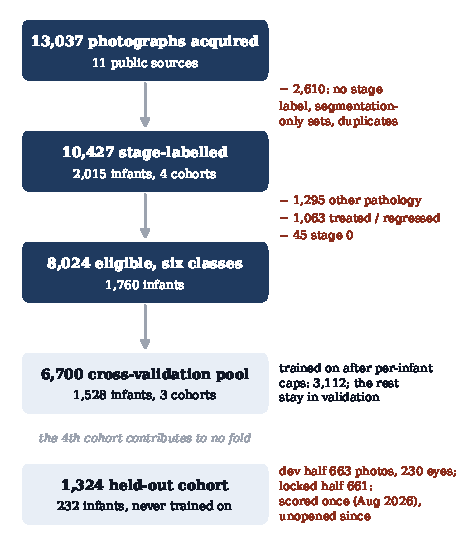
\includegraphics[width=\columnwidth]{fig_cascade.pdf}
\caption{Acquisition cascade. Every exclusion is counted and the reasons sum to the drop (Table~\ref{tab:funnel}). The fourth hospital contributes to no training fold; its locked half was scored once, for the CNN generation, and has not been opened for the transformers.}
\label{fig:cascade}
\end{figure}

\begin{table*}[!t]
\caption{Acquisition cascade in numbers, and how the eligible photographs are used. Removed photographs at the training-eligible step stay in validation: every photograph of the pool is scored exactly once by the model that never trained on its infant.}
\label{tab:funnel}
\centering\scriptsize\setlength{\tabcolsep}{4pt}
\begin{tabular}{@{}lrrr>{\raggedright\arraybackslash}p{7.6cm}@{}}
\toprule
Step & Photos & Infants & Removed & Reason / note\\
\midrule
Acquired & 13{,}037 & -- & -- & 11 publicly released sources \\
Stage-labelled cohorts & 10{,}427 & 2{,}015 & 2{,}610 & no ICROP stage label (plus-only, segmentation sets), too small to fold, re-encoded duplicates \\
Six-class eligible & 8{,}024 & 1{,}760 & 2{,}403 & other pathology 1{,}295, treated 1{,}063, stage 0 45 \\
Cross-validation pool & 6{,}700 & 1{,}528 & -- & three cohorts; every photo in one validation fold \\
Training-eligible & 3{,}112 & 1{,}528 & 3{,}588 & per-infant caps: 2 normal, 20 per disease class; capped photos stay in validation \\
Held-out cohort, dev half & 663 & 116 & -- & 230 eyes; checks and every reported external number \\
Held-out cohort, locked half & 661 & 116 & -- & 230 eyes; opened once, Aug 2026, for the CNN generation \\
\bottomrule
\end{tabular}

\end{table*}

\subsection{Reference standard and label unit}
Labels are those released by the source institutions, graded by their clinicians against ICROP; we did not re-grade, and we state this as the study's principal limitation. The unit a label describes differs by cohort (Table~\ref{tab:sources}) and is respected in every evaluation: Ostrava records one diagnosis per examination session, inherited by every video frame of that session, about \perInfantOstrava{} frames per infant; ROP-VL and Shenzhen label single photographs; the fourth hospital, Multi-View, labels each eye and photographs it in three fixed views. Section~\ref{sec:cnn} shows what this does to a reported number.

\subsection{Splits}
Folds are patient-grouped (five-fold, stratified by class) and shared by every model from the CNN generation onward. Within the \poolImages{}-photograph pool, training keeps at most \capNormal{} normal and \capOther{} disease photographs of any one infant (\trainEligible{} training-eligible photographs; one Ostrava infant alone supplies 470 of the 618 AP-ROP frames), while validation always scores every photograph of the held-out fold. The fourth hospital is held out entirely and split by infant into a development half (\devImages{} photographs, \devEyes{} eyes, \devInfants{} infants), used for checks and for every external number reported here, and a locked half (\lockedImages{} photographs, \lockedEyes{} eyes) opened once, under a protocol committed beforehand, for the CNN generation (\lockedOpened{}) and not read by any code since. \dupExcl{} exact duplicates are excluded from every metric.

\subsection{Shortcut audit}
Five gates run before any model is trained (Table~\ref{tab:audit}): patient leakage across folds; exact and perceptual duplicate leakage; whether the hospital can be decoded from trivial metadata (balanced accuracy \siteDecodable{} against chance 0.333, which names the confound rather than removing it); a metadata-only classifier that uses no pixels, whose macro-F1 of \metaFloorCV{} is the floor every image model must clear; and a disease-controlled probe of site information in the learned features. On the earlier binary split, image dimensions alone, a perfect proxy for the camera, reached AUC \shortcutAUC{}: the shortcut is measured, not hypothetical.

\begin{table}[!t]
\caption{Shortcut audit, run before training on the staging corpus. G3 names a confound that cannot be removed from the data; G4 sets the floor; G5 is reported per model.}
\label{tab:audit}
\centering\scriptsize\setlength{\tabcolsep}{3pt}
\begin{tabular}{@{}l>{\raggedright\arraybackslash}p{4.5cm}>{\raggedright\arraybackslash}p{3.1cm}@{}}
\toprule
Gate & What it measures & Result\\
\midrule
G1 & Patient leakage across folds & none \\
G2 & Exact (MD5) and perceptual (256-bit dHash) duplicate leakage & 0 / 0 pairs; closest distance 15 \\
G3 & Site decodable from trivial metadata (balanced accuracy; chance) & 0.997 (chance 0.333); stage 4/5 exists in one source only \\
G4 & Metadata-only classifier, no pixels (macro-F1 floor) & CV 0.187, unseen hospital 0.062 \\
G5 & Disease-controlled site probe on embeddings & per model; not run for A--I (reported for the CNN generation in~\cite{nagpure2026}) \\
-- & Image dimensions alone, earlier binary split (AUC) & 0.911 \\
\bottomrule
\end{tabular}

\end{table}

\subsection{Preprocessing}
Every model from the CNN generation onward sees the same input (Fig.~\ref{fig:preprocess}): the retinal disc is cropped from the camera frame, letterboxed to a square, contrast-enhanced with CLAHE~\cite{zuiderveld1994} on the luminance channel (clip 2.0, $8\times8$ tiles), resized (392~px for the transformers, 384~px for EfficientNetV2-S) and normalised. Preprocessing is applied identically at training, validation, testing and in the served application. Augmentation at training time adds flips, rotation, colour jitter and a site-randomising colour transform; it never changes the test-time pipeline.

\begin{figure*}[!t]
\centering
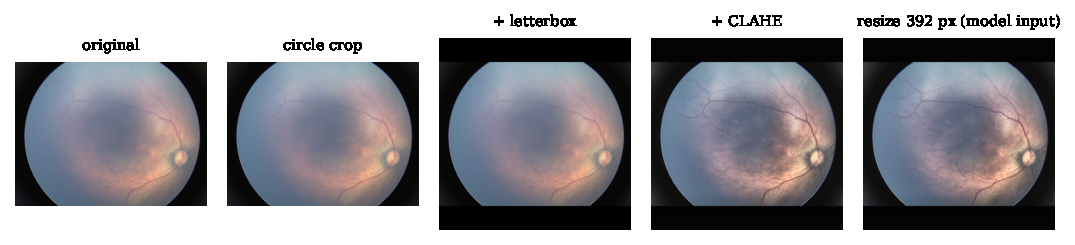
\includegraphics[width=\textwidth]{fig_preprocess.pdf}
\caption{Preprocessing of one development-half photograph: circle crop, letterbox to a square, CLAHE on the luminance channel, resize to the model input. The same steps run in the served application.}
\label{fig:preprocess}
\end{figure*}

\section{Stage 1: Classical Machine Learning}\label{sec:ml}
Classical learners served two purposes in this project: as audit probes, and as the baseline against which the deep models are read.

\textbf{Audit probes.} Logistic regression and a random forest~\cite{breiman2001} on image width and height alone predicted ROP with AUC \shortcutAUC{} on the first binary split (Section~\ref{sec:data}): the three Ostrava cameras photograph different populations, and the camera is written into the image size. On the staging corpus the same learners, given only metadata, reach macro-F1 \metaFloorCV{} in cross-validation and \metaFloorDev{} at the unseen hospital (Table~\ref{tab:audit}).

\textbf{Hand-crafted features.} An independent package trained by a team member turns each photograph, after a black-border crop, resize to 256~px and CLAHE, into \mateMLFeat{} numbers: colour statistics and HSV histograms, local binary patterns~\cite{ojala2002}, grey-level co-occurrence statistics~\cite{haralick1973}, histograms of oriented gradients~\cite{dalal2005} and Frangi vesselness statistics~\cite{frangi1998}. Twelve learners were trained on them (support-vector machine~\cite{cortes1995}, $k$-nearest neighbours, random forest and extra trees~\cite{breiman2001}, XGBoost~\cite{chen2016}, LightGBM~\cite{ke2017}, CatBoost~\cite{prokhorenkova2018}, histogram gradient boosting, logistic regression, a multilayer perceptron, and soft-voting and stacking ensembles of the three best by five-fold cross-validation accuracy), on \mateN{} of this project's photographs in four classes (normal, stage 1, 2, 3) split 80/20 \emph{by photograph}. Table~\ref{tab:mateml} gives every learner; the best, \mateMLBest{}, reaches test accuracy \mateMLAcc{} and QWK \mateMLQ{} on \mateMLTest{} photographs. Because the split is by photograph, \mateLeakTest{} of its test photographs share an infant with its training set (Table~\ref{tab:matedata}), so even these modest numbers are optimistic; they are the classical ceiling on this corpus, not a benchmark result.

\begin{table}[!t]
\caption{Classical learners on \mateMLFeat{} hand-crafted features (independent package; four classes; photo-level 80/20 split; CV: five-fold accuracy on the augmented training rows, which ranked the learners; s: training seconds). \emph{Caveat}: photo-level split (Section~\ref{sec:mate}).}
\label{tab:mateml}
\centering\scriptsize\setlength{\tabcolsep}{3pt}
\begin{tabular}{@{}lccccccr@{}}
\toprule
 & CV & \multicolumn{5}{c}{Test, 629 photographs} & \\
\cmidrule(lr){3-7}
Model & Acc. & Acc. & Bal.\,acc. & mF1 & QWK & AUC & s\\
\midrule
SVM (RBF) & 0.562 & 0.585 & 0.576 & 0.576 & 0.547 & 0.812 & 23 \\
Soft Voting (top-3) & 0.571 & 0.585 & 0.571 & 0.569 & 0.573 & 0.810 & 593 \\
Extra Trees & 0.542 & 0.574 & 0.561 & 0.555 & 0.502 & 0.790 & 6 \\
XGBoost & 0.562 & 0.568 & 0.554 & 0.552 & 0.535 & 0.804 & 130 \\
HistGradBoost & 0.566 & 0.568 & 0.552 & 0.550 & 0.551 & 0.807 & 459 \\
LightGBM & 0.567 & 0.566 & 0.555 & 0.555 & 0.563 & 0.810 & 39 \\
MLP & 0.534 & 0.558 & 0.547 & 0.549 & 0.531 & 0.795 & 13 \\
Stacking (top-3) & 0.567 & 0.556 & 0.543 & 0.541 & 0.556 & 0.807 & 2{,}107 \\
Random Forest & 0.540 & 0.555 & 0.540 & 0.532 & 0.500 & 0.786 & 9 \\
CatBoost & 0.547 & 0.522 & 0.511 & 0.508 & 0.458 & 0.784 & 33 \\
KNN & 0.518 & 0.501 & 0.493 & 0.489 & 0.403 & 0.736 & 5 \\
Logistic Reg. & 0.520 & 0.488 & 0.477 & 0.475 & 0.410 & 0.762 & 6 \\
\bottomrule
\end{tabular}

\end{table}

\section{Stage 2: Convolutional Networks}\label{sec:cnn}
\subsection{A binary screener and the device shortcut}
The project's first model (June 2026) was an EfficientNet-B3~\cite{tan2019} shared between ROP yes/no and diabetic retinopathy under an image-level split: ROP test accuracy \vOneAcc{}, F1 \vOneFone{} (Table~\ref{tab:v1}). A sweep of five ImageNet CNNs (EfficientNet-B0, EfficientNetV2-S~\cite{tan2021}, MobileNetV3-L~\cite{howard2019}, ResNet50~\cite{he2016}, DenseNet121~\cite{huang2017}) for binary ROP on Ostrava chose ResNet50 by validation AUC (\sweepValAUC{}; test \sweepAUC{}), and ResNet50 was deployed as the screening head (Table~\ref{tab:sweep}). The audit then showed that image dimensions alone scored AUC \shortcutAUC{} on the same split, because every ROP-positive test image came from one camera. Scored at the fourth hospital with its deployed threshold unchanged, the lowest score the head assigned any photograph exceeded its own decision threshold: it flagged all 663 development-half photographs, including every healthy eye, for specificity 0.000 and AUC 0.691~\cite{nagpure2026}. The head was retired. This is the documented failure mode of cross-camera transfer~\cite{chen2021}, and it is invisible to any internal metric.

\begin{table}[!t]
\caption{First model (June 2026): EfficientNet-B3, one shared model for binary ROP and diabetic retinopathy (DR), image-level split. P / R: precision / recall. \emph{Caveat}: image-level split and two diseases in one model; retired.}
\label{tab:v1}
\centering\scriptsize\setlength{\tabcolsep}{2.0pt}
\begin{tabular}{@{}>{\raggedright\arraybackslash}p{1.45cm}rccccc@{}}
\toprule
Split & n & Acc. & mF1 & No ROP P / R & ROP P / R & ROP F1\\
\midrule
ROP val & 928 & 0.647 & 0.646 & 0.476 / 0.933 & 0.941 / 0.510 & 0.661 \\
ROP test & 1{,}502 & 0.733 & 0.731 & 0.644 / 0.913 & 0.891 / 0.585 & 0.706 \\
DR val, ep.\ 5 & -- & 0.719 & 0.497 & -- & -- & -- \\
\bottomrule
\end{tabular}

\end{table}

\begin{table}[!t]
\caption{June 2026 binary CNN sweep (ROP yes/no, Ostrava, sweep validation split; QWK$_2$ binary kappa) and, $^\ast$, the deployed ResNet50 on its own validation and test split. \emph{Caveat}: inflated by the device shortcut (image size alone: AUC \shortcutAUC{}).}
\label{tab:sweep}
\centering\scriptsize\setlength{\tabcolsep}{2.2pt}
\begin{tabular}{@{}lcccccc@{}}
\toprule
Architecture & Acc. & mF1 & QWK$_2$ & AUC & Params (M) & CPU ms\\
\midrule
efficientnet\_b0 & 0.758 & 0.757 & 0.525 & 0.867 & 4.01 & 56.2 \\
efficientnet\_v2\_s & 0.706 & 0.701 & 0.431 & 0.870 & 20.18 & 130.1 \\
mobilenet\_v3\_large & 0.744 & 0.743 & 0.500 & 0.857 & 4.2 & 34.4 \\
resnet50 & 0.886 & 0.882 & 0.766 & 0.964 & 23.51 & 157.2 \\
densenet121 & 0.764 & 0.764 & 0.537 & 0.887 & 6.96 & 136 \\
\midrule
resnet50$^\ast$ val & 0.747 & 0.740 & 0.499 & 0.842 & -- & -- \\
resnet50$^\ast$ test & 0.844 & 0.843 & 0.688 & 0.927 & -- & -- \\
\bottomrule
\end{tabular}

\end{table}

\subsection{Six-class staging with patient-grouped folds}
The second generation (August 2026) moved to six-class ICROP-3 staging on the audited corpus with patient-grouped five-fold cross-validation and the held-out hospital. All arms share an ImageNet-initialised EfficientNetV2-S backbone and the preprocessing of Fig.~\ref{fig:preprocess}. A \emph{structured} head combined a CORN ordinal branch~\cite{corn2023} over the stages (AP-ROP masked from the ordinal loss), an independent AP-ROP sigmoid branch and a domain-adversarial site head~\cite{ganin2016}; the \emph{flat} baseline is a six-way softmax. Both trained at natural class prevalence for a fixed epoch budget with last-epoch weights, never a validation-selected checkpoint. Two findings shaped everything after (Table~\ref{tab:v2}; details in~\cite{nagpure2026}).

\textbf{The architectures were indistinguishable.} Under cross-validation the structured and flat heads differed by $-0.006$ macro-F1 at one seed and $+0.022$ at the other: opposite signs, an order of magnitude inside the per-fold spread. A single fold had shown the structured head failing on AP-ROP across five backbones; it dissolved under cross-validation, because that fold's validation split held the one heavily imaged, session-labelled infant.

\textbf{The evaluation unit decided the result.} On the locked half, scored once, the same predictions gave QWK \vTwoLockedImgQ{} per photograph and \vTwoLockedEyeQ{} per eye (accuracy \vTwoLockedEyeAcc{}) for the structured head at seed \seedA{}, and the gap of 0.23--0.28 held in all four arm--seed cells. The mechanism is anatomical: the ROP ridge grows in the retinal periphery, so a posterior-pole frame of a diseased eye is, as a picture, normal, and frames inherit the eye's or session's label. Posterior-pole frames of diseased eyes were called normal 71.7\% of the time against 12.7\% for temporal frames~\cite{nagpure2026}. From this point every eye-level result in the project uses the clinical reading rule: an eye is staged by its most severe photograph.

\begin{table*}[!t]
\caption{Second generation (August 2026): EfficientNetV2-S structured head (CORN ordinal + AP-ROP branch + site adversary, \vtStructParams{} parameters) versus a flat softmax, natural sampling, five-fold patient-grouped CV. QWK$_6$: legacy six-class definition; QWK5$_d$: rows with true or predicted AP-ROP removed; QWK5: the definition used for the transformers (AP-ROP folded onto stage 4/5). Dev and locked: the unseen hospital; eye = most severe photograph; locked half opened once (\lockedOpened{}). \emph{Caveat}: own checkpoint rule and QWK definitions; the flat arm is re-scored as arm C in Table~\ref{tab:headline}.}
\label{tab:v2}
\centering\scriptsize\setlength{\tabcolsep}{3.4pt}
\begin{tabular}{@{}ll@{\hspace{4pt}}cccccc@{\hspace{5pt}}c@{\hspace{5pt}}cc@{\hspace{5pt}}ccc@{}}
\toprule
 & & \multicolumn{6}{c}{CV pooled OOF, 6{,}700 photos} & Dev & \multicolumn{2}{c}{Locked, photo} & \multicolumn{3}{c}{Locked, eye (max)}\\
\cmidrule(lr){3-8}\cmidrule(lr){9-9}\cmidrule(lr){10-11}\cmidrule(l){12-14}
Head & Seed & QWK$_6$ & QWK5$_d$ & QWK5 & Acc. & mF1 & AUC & QWK5 & QWK5$_d$ & QWK5 & QWK5$_d$ & QWK5 & Acc.\\
\midrule
Structured & 42 & 0.761 & 0.897 & 0.807 & 0.786 & 0.652 & 0.969 & 0.755 & 0.473 & 0.517 & 0.813 & 0.823 & 0.646 \\
 & 1337 & 0.783 & 0.905 & 0.824 & 0.804 & 0.666 & 0.967 & 0.752 & 0.456 & 0.500 & 0.794 & 0.808 & 0.627 \\
Flat & 42 & 0.777 & 0.897 & 0.820 & 0.789 & 0.655 & 0.968 & 0.756 & 0.492 & 0.551 & 0.808 & 0.823 & 0.635 \\
 & 1337 & 0.770 & 0.898 & 0.813 & 0.787 & 0.658 & 0.966 & 0.764 & 0.486 & 0.543 & 0.801 & 0.818 & 0.630 \\
\bottomrule
\end{tabular}

\end{table*}

\subsection{An independent CNN package on a photo-level split}
The same team member's second package fine-tuned six ImageNet CNNs (ResNet50, DenseNet121, EfficientNet-B2, ConvNeXt-Tiny~\cite{liu2022}, ResNeSt-50d~\cite{zhang2022}, MobileNetV3-L; timm weights~\cite{wightman2019}, 224~px, head warm-up then full fine-tuning, AdamW~\cite{loshchilov2019}, cosine schedule, class-weighted cross-entropy with label smoothing, early stopping on validation macro-F1, flip test-time augmentation) on the same four-class photographs, split 80/10/10 by photograph (Table~\ref{tab:matecnn}). The best, \mateCNNBest{}, reached test accuracy \mateCNNAcc{} and QWK \mateCNNQ{}; \mateCNNDiverged{} diverged (\mateCNNDivergedAcc{}); a soft vote of the three best by validation macro-F1 gave \mateCNNEnsAcc{}. Read beside Table~\ref{tab:v2}, these numbers show what the split does: four classes instead of six, same-hospital test photographs sharing infants with training, and no external hospital raise a CNN's accuracy from the 0.5--0.6 range of the audited protocol into the 0.8 range, without the model learning anything new.

\begin{table}[!t]
\caption{Independent CNN package: ImageNet-pretrained CNNs (timm), 224~px, up to 40 epochs with early stopping on validation macro-F1; the soft vote averages the three with the highest validation macro-F1. Four classes; photo-level split (Section~\ref{sec:mate}).}
\label{tab:matecnn}
\centering\scriptsize\setlength{\tabcolsep}{1.9pt}
\begin{tabular}{@{}lccc@{\hspace{6pt}}ccccc@{}}
\toprule
 & & & Val & \multicolumn{5}{c}{Test, 315 photographs}\\
\cmidrule(l){5-9}
Model & Par.\,(M) & Ep. & mF1 & Acc. & Bal. & mF1 & QWK & AUC\\
\midrule
resnest50d & 25.4 & 32 & 0.821 & 0.835 & 0.827 & 0.828 & 0.898 & 0.956 \\
densenet121 & 7.0 & 36 & 0.822 & 0.822 & 0.816 & 0.815 & 0.880 & 0.942 \\
efficientnet\_b2 & 7.7 & 40 & 0.832 & 0.819 & 0.812 & 0.811 & 0.884 & 0.943 \\
resnet50 & 23.5 & 40 & 0.827 & 0.810 & 0.802 & 0.800 & 0.860 & 0.951 \\
mobilenetv3\_large\_100 & 4.2 & 22 & 0.769 & 0.775 & 0.775 & 0.769 & 0.840 & 0.925 \\
convnext\_tiny & 27.8 & 13 & 0.491 & 0.530 & 0.546 & 0.520 & 0.497 & 0.821 \\
\midrule
Soft vote, top 3 & -- & -- & 0.856 & 0.825 & 0.821 & 0.818 & 0.881 & 0.959 \\
\bottomrule
\end{tabular}

\end{table}

\section{Stage 3: Vision Transformers}\label{sec:vit}
\subsection{Pre-registration}
A protocol fixing the arms, parity rules, label units, selection rule, primary and secondary endpoints, bootstrap, duplicate exclusion and minimum detectable difference was committed to version control (\texttt{\protoCommit}, \protoDate{}) before any transformer was trained; \nAmend{} dated amendments, each committed before the experiment it governs and the last on \lastAmendDate{}, added probe-chosen learning rates and later arms. No selection used the unseen hospital. The primary endpoint, locked-half eye-level QWK for the contrast A$-$C, is unscored: the locked half will be opened once, for all nine arms together, after approval.

\subsection{Arms}
All nine arms share the preprocessing of Fig.~\ref{fig:preprocess}, class-balanced cross-entropy ($\beta=0.999$)~\cite{cui2019} with label smoothing, strong and site-randomising augmentation, batch 16, 20 epochs, AdamW, a one-cycle cosine schedule, mixed precision, last-epoch weights without early stopping, and seeds \seedA{} and \seedB{} (Table~\ref{tab:recipe}). Only the backbone, input size, normalisation and learning-rate recipe may differ. \textbf{A}, retinal: RETFound-Green ViT-S/14 with register tokens~\cite{engelmann2025}, a fresh six-way head. \textbf{B}, natural: DINOv2 ViT-S/14-reg~\cite{oquab2024,dosovitskiy2021}, the identical architecture, so that pre-training domain is the only difference between A and B. \textbf{C}: the flat EfficientNetV2-S of Section~\ref{sec:cnn}, re-scored from its saved predictions under the new rules. \textbf{D}: B trained with a log-sum-exp loss over up to eight frames of each Ostrava session, scored against the session label, so that the loss sees the unit the label describes. \textbf{E}: the mean of A, B and C. \textbf{F}: B with self-ensembling adaptation~\cite{french2018} on unlabelled photographs of the unseen hospital's development half (its development numbers are therefore transductive). \textbf{G}: B at DINOv2's native 518~px. \textbf{H}: B's recipe on a cleaned pool (\vfourTrain{} training photographs after a per-camera Ostrava frame-quality rule, cap re-ranking by sharpness and near-duplicate removal). \textbf{I}: H plus a regularising recipe fixed in the amendment (weight EMA, head warm-up, wider rotation and crop, gamma and noise jitter, a Fourier amplitude swap, label smoothing 0.10). Transformers use layer-wise learning-rate decay 0.8, drop-path 0.1 and head dropout 0.3; the peak learning rate was chosen per arm by a probe on an inner patient-disjoint split of one fold's training rows. All sessions ran on Kaggle \gpu{} GPUs, about \BfoldMinutes{}~min per fold for B.

\begin{table*}[!t]
\caption{Recipe and cost of the transformer arms. Shared by every trained arm: circle-crop, letterbox, CLAHE; class-balanced cross-entropy; strong and site-randomising augmentation; batch 16; AdamW; one-cycle cosine schedule; last-epoch weights. LLRD: layer-wise learning-rate decay; LS: label smoothing. Cost: mean over CV folds and both seeds on Kaggle \gpu{} GPUs; C and E were not trained in this generation.}
\label{tab:recipe}
\centering\scriptsize\setlength{\tabcolsep}{3pt}
\begin{tabular}{@{}llcllcccc>{\raggedright\arraybackslash}p{6.2cm}cc@{}}
\toprule
Arm & Backbone & px & Norm. & Pool & Peak lr & LLRD & LS & Ep. & Differences from B's recipe & min/fold & img/s\\
\midrule
A & \texttt{retfound\_green} & 392 & half & v3 & 2e-4 & 0.8 & 0.05 & 20 & RETFound-Green weights & 32.1 & 38.6 \\
\textbf{B} & \texttt{dinov2\_s} & 392 & imagenet & v3 & 1e-4 & 0.8 & 0.05 & 20 & reference recipe & 33.3 & 31.9 \\
C & \texttt{effnetv2s} & 384 & imagenet & v3 & 3e-4 & -- & 0.05 & 20 & v2 flat softmax, natural sampler; saved predictions re-scored & -- & -- \\
D & \texttt{dinov2\_s} & 392 & imagenet & v3 & 1e-4 & 0.8 & 0.05 & 20 & LSE bag loss on Ostrava sessions, $K{=}8$, $\tau{=}1$ & 32.5 & 29.0 \\
E & -- & -- & -- & v3 & -- & -- & -- & -- & mean of A, B, C probabilities, matched by seed; no training & -- & -- \\
F$^\dagger$ & \texttt{dinov2\_s} & 392 & imagenet & v3 & 1e-4 & 0.8 & 0.05 & 20 & self-ensembling on unlabelled dev photos, EMA 0.99, conf.\ $\ge$0.9 & 61.7 & 14.2 \\
G & \texttt{dinov2\_s} & 518 & imagenet & v3 & 1e-4 & 0.8 & 0.05 & 20 & 518 px & 58.1 & 19.2 \\
H & \texttt{dinov2\_s} & 392 & imagenet & v4 & 1e-4 & 0.8 & 0.05 & 20 & v4 pool (per-device quality filter) & 34.1 & 31.2 \\
I & \texttt{dinov2\_s} & 392 & imagenet & v4 & 1e-4 & 0.8 & 0.1 & 20 & EMA weights 0.999; 1 head-only epoch; label smoothing 0.1; rot.\ $\pm$180$^\circ$, crop $\ge$0.85, gamma, noise, Fourier swap $p\,0.5$ & 34.8 & 32.1 \\
\bottomrule
\end{tabular}

\end{table*}

\subsection{Eye-level inference, endpoints and statistics}
Each photograph receives a probability vector; an eye's stage is the most severe predicted stage over its photographs, the photograph attaining it is the driving photograph, and its vector is the eye's vector; the eye's any-ROP score is $\max_i(1-p_{i,\mathrm{normal}})$. The selection rule is cross-validation pooled out-of-fold QWK per photograph on the five-class map (AP-ROP folded onto stage 4/5), computed once per arm; the v4 round could replace B only if H or I beat it by at least \marginCV{} QWK in cross-validation while staying within \marginLOSO{} of it on a leave-one-source-out (LOSO) guard. QWK is quadratic-weighted kappa~\cite{cohen1968}; we also report unweighted kappa because the human literature does. Intervals are 95\% percentile bootstrap over \nReps{} resamples of infants, with each arm's prediction lists (two seeds; ten fold checkpoints at the unseen hospital) averaged inside each replicate; paired contrasts use the same resample. Calibration is measured as expected calibration error (ECE)~\cite{guo2017} of the eye's driving-photograph probability vector. The screening operating point is the largest any-ROP threshold that keeps cross-validation unit-level sensitivity at or above 0.90, carried unchanged to the unseen hospital.

\subsection{An independent foundation-model package}
The team member's third package kept a RETFound-DINOv2 ViT-L/14 backbone~\cite{zhou2023} frozen (\mateFMtotal{}~M weights) and trained LoRA adapters~\cite{hu2022} of rank 16 on the attention and MLP projections of all 24 blocks plus a linear head (\mateFMtrainable{}~M trainable), bf16, four-view flip test-time augmentation, on the same four-class photo-level split; a sweep of one change each (10 epochs) chose a 280-px variant on validation, trained for 30 epochs with three seeds (Table~\ref{tab:matefm}).

\begin{table*}[!t]
\caption{Independent foundation-model package: RETFound-DINOv2 ViT-L/14 frozen, LoRA adapters (rank 16, alpha 32 unless stated) on attention and MLP layers, linear four-class head; best epoch by validation macro-F1; four-view flip TTA. Probes: 10 epochs, one change each. Four classes; photo-level split (Section~\ref{sec:mate}).}
\label{tab:matefm}
\centering\scriptsize\setlength{\tabcolsep}{3.4pt}
\begin{tabular}{@{}l>{\raggedright\arraybackslash}p{3.3cm}ccc@{\hspace{5pt}}c@{\hspace{6pt}}ccccc@{}}
\toprule
 & & Trainable & & & Val & \multicolumn{5}{c}{Test, 315 photographs}\\
\cmidrule(l){7-11}
Run & Change & (M) & px & Epochs & mF1 & Acc. & Bal.\,acc. & mF1 & QWK & AUC\\
\midrule
\multicolumn{11}{@{}l}{\emph{Stage-2 probes, 10 epochs, seed 42 (one change each vs the first row)}}\\
p mlp & LoRA on attention + MLP (probe base) & 6.30 & 224 & 10 & 0.810 & 0.797 & 0.798 & 0.792 & 0.862 & 0.947 \\
p mlp r32 & rank 32, alpha 64 & 12.59 & 224 & 10 & 0.819 & 0.816 & 0.811 & 0.810 & 0.867 & 0.950 \\
p mlp dp1 & drop-path 0.1 & 6.30 & 224 & 10 & 0.830 & 0.797 & 0.799 & 0.793 & 0.861 & 0.951 \\
p mlp lr6e4 & lr 6e-4 & 6.30 & 224 & 10 & 0.829 & 0.829 & 0.825 & 0.823 & 0.897 & 0.958 \\
p mlp img280 & 280 px input & 6.30 & 280 & 10 & 0.834 & 0.822 & 0.821 & 0.818 & 0.875 & 0.959 \\
p mlp ord & ordinal auxiliary loss 0.3 & 6.30 & 224 & 10 & 0.807 & 0.806 & 0.807 & 0.803 & 0.876 & 0.951 \\
p mlp combo & r32 + dp 0.1 + lr 6e-4 + 280 px & 12.59 & 280 & 10 & 0.623 & 0.651 & 0.662 & 0.617 & 0.761 & 0.900 \\
\midrule
\multicolumn{11}{@{}l}{\emph{Full-length runs, 30 epochs max}}\\
final base s42 & attention-only LoRA, 30 ep & 2.37 & 224 & 30 & 0.817 & 0.825 & 0.818 & 0.818 & 0.900 & 0.956 \\
final mlp s42 & attention + MLP, 224 px, 30 ep & 6.30 & 224 & 25 & 0.816 & 0.778 & 0.763 & 0.765 & 0.860 & 0.948 \\
final mlp img280 s42 & chosen config, seed 42 & 6.30 & 280 & 25 & 0.846 & 0.787 & 0.787 & 0.779 & 0.870 & 0.950 \\
final mlp img280 s1 & chosen config, seed 1 & 6.30 & 280 & 30 & 0.841 & 0.822 & 0.818 & 0.815 & 0.888 & 0.952 \\
final mlp img280 s2 & chosen config, seed 2 & 6.30 & 280 & 30 & 0.846 & 0.832 & 0.827 & 0.826 & 0.889 & 0.951 \\
\midrule
3 seeds averaged & chosen config, seeds 42, 1, 2 & -- & -- & -- & 0.839 & 0.844 & 0.842 & 0.839 & 0.900 & 0.964 \\
3 seeds + 4 CNNs & plus EffNet-B2, ResNet50, DenseNet121, ResNeSt-50d & -- & -- & -- & 0.863 & 0.860 & 0.859 & 0.855 & 0.908 & 0.972 \\
\bottomrule
\end{tabular}

\end{table*}

\section{Results}\label{sec:results}
\subsection{The transformer arms}
Table~\ref{tab:headline} and Fig.~\ref{fig:selection} give the nine arms. The selection rule chose B: cross-validation QWK \BcvQ{} \BcvQci{}, accuracy \BcvAcc{}, any-ROP AUC \BcvAUC{}, unweighted kappa \BkappaU{}. At the unseen hospital, per eye, B scores QWK \BdevQ{} \BdevQci{}, accuracy \BdevAcc{}, macro-F1 \BdevMF{}, any-ROP AUC \BdevAUC{}, unweighted kappa \BdevKappaU{} (Fig.~\ref{fig:dev}). The retinal-versus-natural contrast A$-$B was \cvDiffAB{} \cvDiffABci{} in cross-validation and \devDiffAB{} \devDiffABci{} per eye at the unseen hospital: the sign reverses between the training hospitals and the unseen one and neither interval clears the minimum detectable difference. The transformer-versus-CNN contrast A$-$C was \devDiffAC{} \devDiffACci{} per eye. Neither v4 arm met the adoption rule: in cross-validation I$-$B was \cvDiffIB{} \cvDiffIBci{} and H$-$B \cvDiffHB{} \cvDiffHBci{}, both intervals wholly below the $+$\marginCV{} bar, while both passed the LOSO guard (Fig.~\ref{fig:loso}). At the unseen hospital I scored I$-$B \devDiffIB{} \devDiffIBci{}, the one descriptive gain, in QWK only and below the detectable difference; it is not the served model.

\begin{table*}[!t]
\caption{Transformer generation: headline results, all arms, both seeds pooled. CV: pooled out-of-fold, per photograph. Dev: unseen hospital, development half, per eye. QWK5 with 95\% infant-clustered CI; Acc.\ six-class accuracy; Bal.\,acc.\ mean per-class recall; mF1 macro-F1 over present classes; AUC and AP: any ROP vs normal. Bold letter: selected arm. $^\dagger$Transductive: saw the dev photographs unlabelled in training.}
\label{tab:headline}
\centering\scriptsize\setlength{\tabcolsep}{3.3pt}
\begin{tabular}{@{}ll@{\hspace{4pt}}lcccc@{\hspace{6pt}}lcccc@{}}
\toprule
 & & \multicolumn{5}{c}{CV, per photograph (6{,}686 photos)} & \multicolumn{5}{c}{Unseen hospital, dev half, per eye (230 eyes)}\\
\cmidrule(lr){3-7}\cmidrule(l){8-12}
Arm & Model & QWK5 [95\% CI] & Acc. & Bal.\,acc. & mF1 & AUC & QWK5 [95\% CI] & Acc. & mF1 & AUC & AP\\
\midrule
A & RETFound-Green ViT-S & 0.794 [0.664, 0.915] & 0.759 & 0.656 & 0.643 & 0.977 & 0.774 [0.707, 0.828] & 0.632 & 0.563 & 0.935 & 0.984 \\
\textbf{B} & DINOv2 ViT-S & 0.825 [0.737, 0.911] & 0.766 & 0.674 & 0.653 & 0.979 & 0.756 [0.679, 0.821] & 0.630 & 0.566 & 0.937 & 0.984 \\
C & EfficientNetV2-S (baseline) & 0.816 [0.713, 0.916] & 0.788 & 0.672 & 0.656 & 0.967 & 0.760 [0.680, 0.822] & 0.624 & 0.573 & 0.943 & 0.986 \\
D & DINOv2 + exam-level loss & 0.797 [0.699, 0.909] & 0.803 & 0.671 & 0.661 & 0.942 & 0.746 [0.671, 0.810] & 0.609 & 0.542 & 0.935 & 0.984 \\
E & Ensemble A+B+C & 0.821 [0.708, 0.927] & 0.787 & 0.680 & 0.664 & 0.981 & 0.770 [0.697, 0.827] & 0.639 & 0.568 & 0.944 & 0.986 \\
F$^\dagger$ & DINOv2 + adaptation & 0.812 [0.704, 0.915] & 0.761 & 0.663 & 0.644 & 0.980 & 0.744 [0.665, 0.812] & 0.624 & 0.552 & 0.940 & 0.985 \\
G & DINOv2 at 518 px & 0.814 [0.706, 0.915] & 0.764 & 0.667 & 0.647 & 0.984 & 0.767 [0.697, 0.827] & 0.627 & 0.551 & 0.939 & 0.985 \\
H & DINOv2 on the v4 pool & 0.813 [0.707, 0.914] & 0.765 & 0.660 & 0.646 & 0.982 & 0.750 [0.674, 0.814] & 0.620 & 0.556 & 0.941 & 0.985 \\
I & DINOv2, v4 pool + v4 recipe & 0.821 [0.727, 0.912] & 0.750 & 0.645 & 0.618 & 0.982 & 0.776 [0.705, 0.834] & 0.633 & 0.561 & 0.944 & 0.986 \\
\bottomrule
\end{tabular}

\end{table*}

\begin{figure}[!t]
\centering
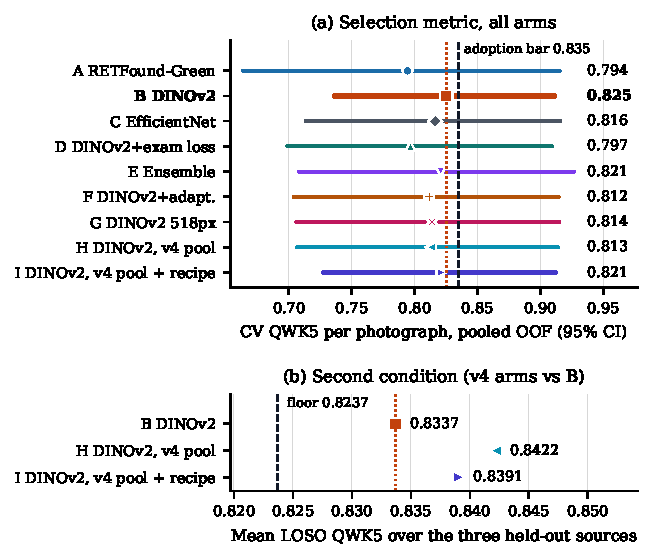
\includegraphics[width=\columnwidth]{fig_selection.pdf}
\caption{Selection. (a) CV QWK5 per photograph, pooled out-of-fold, 95\% CI; dotted: B; dashed: the adoption bar (B $+$ \marginCV{}) a v4 arm had to reach. (b) The LOSO guard: mean QWK5 over three held-out sources at least B $-$ \marginLOSO{} (dashed).}
\label{fig:selection}
\end{figure}

\begin{figure}[!t]
\centering
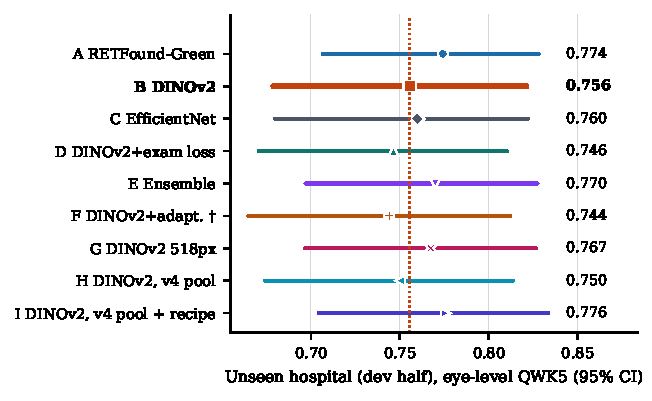
\includegraphics[width=\columnwidth]{fig_dev_eye.pdf}
\caption{Unseen hospital, development half: eye-level QWK5 with 95\% CI, \devLists{} fold--seed models per arm. Descriptive; no selection used it. $^\dagger$Transductive.}
\label{fig:dev}
\end{figure}

\begin{figure}[!t]
\centering
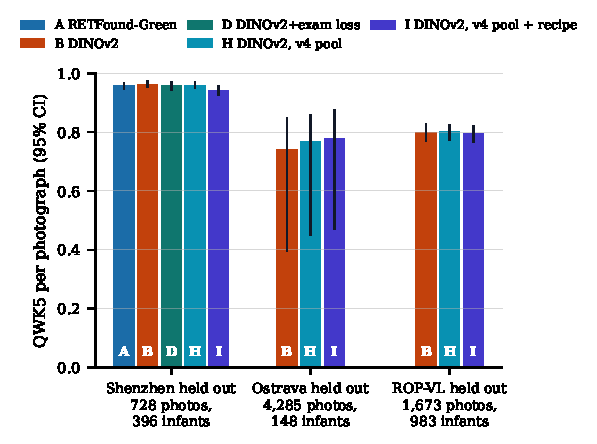
\includegraphics[width=\columnwidth]{fig_loso.pdf}
\caption{Leave-one-source-out: each model trains on two cohorts and scores every photograph of the third (both seeds pooled). Stage 4/5 exists only in ROP-VL, so that fold scores it untrained.}
\label{fig:loso}
\end{figure}

\subsection{Where the errors are}
Table~\ref{tab:stage} and Figs.~\ref{fig:stage}--\ref{fig:cm} place the errors. For B at the unseen hospital, per eye, recall is \BdevRecNormal{} for normal, \BdevRecStageOne{} for stage 1, \BdevRecStageTwo{} for stage 2 and \BdevRecStageThree{} for stage 3; errors are between adjacent stages (normal/stage 1 and stage 1/stage 2), where human readers also disagree most~\cite{gschliesser2015,campbell2016}, and two-stage errors are rare. In cross-validation recall is \BcvRecNormal{}, \BcvRecStageOne{}, \BcvRecStageTwo{}, \BcvRecStageThree{}, \BcvRecStageFourFive{} and \BcvRecArop{} for the six classes; the low AP-ROP figure is dominated by the one infant whose 470 frames carry one examination label. The transformers gain on stage 1 over the CNN at the unseen hospital (recall about 0.5 against 0.4). Stage 4/5 and AP-ROP have five and two eyes at the unseen hospital and are reported as not externally validated.

\begin{table*}[!t]
\caption{Recall / precision per class, both seeds pooled. Upper block: CV per photograph; lower block: unseen hospital (dev half) per eye. Class counts in each block's header. S: stage; AP: AP-ROP.}
\label{tab:stage}
\centering\scriptsize\setlength{\tabcolsep}{5pt}
\begin{tabular}{@{}lcccccc@{}}
\toprule
Arm & Normal & Stage 1 & Stage 2 & Stage 3 & Stage 4/5 & AP-ROP\\
\midrule
\multicolumn{7}{@{}l}{\emph{CV, per photograph; n photos: Normal 3{,}837, S1 574, S2 952, S3 617, S4/5 89, AP 617}}\\
A & 0.912 / 0.947 & 0.569 / 0.293 & 0.584 / 0.541 & 0.725 / 0.848 & 0.876 / 0.741 & 0.268 / 0.760 \\
\textbf{B} & 0.909 / 0.959 & 0.583 / 0.302 & 0.561 / 0.583 & 0.722 / 0.788 & 0.882 / 0.668 & 0.389 / 0.705 \\
C & 0.951 / 0.932 & 0.497 / 0.369 & 0.604 / 0.565 & 0.724 / 0.810 & 0.876 / 0.596 & 0.382 / 0.801 \\
D & 0.993 / 0.893 & 0.475 / 0.582 & 0.488 / 0.646 & 0.712 / 0.772 & 0.865 / 0.553 & 0.490 / 0.581 \\
E & 0.943 / 0.949 & 0.551 / 0.346 & 0.620 / 0.570 & 0.729 / 0.847 & 0.910 / 0.684 & 0.328 / 0.748 \\
F$^\dagger$ & 0.911 / 0.959 & 0.570 / 0.291 & 0.562 / 0.566 & 0.722 / 0.767 & 0.888 / 0.706 & 0.327 / 0.746 \\
G & 0.914 / 0.962 & 0.607 / 0.308 & 0.567 / 0.552 & 0.720 / 0.802 & 0.893 / 0.720 & 0.302 / 0.705 \\
H & 0.924 / 0.952 & 0.570 / 0.326 & 0.557 / 0.520 & 0.725 / 0.807 & 0.876 / 0.740 & 0.306 / 0.682 \\
I & 0.909 / 0.960 & 0.490 / 0.298 & 0.568 / 0.497 & 0.741 / 0.725 & 0.893 / 0.677 & 0.269 / 0.617 \\
\midrule
\multicolumn{7}{@{}l}{\emph{Unseen hospital (dev half), per eye; n eyes: Normal 50, S1 68, S2 46, S3 59, S4/5 5, AP 2}}\\
A & 0.930 / 0.620 & 0.521 / 0.595 & 0.544 / 0.621 & 0.585 / 0.888 & 0.540 / 0.725 & 0.650 / 0.106 \\
\textbf{B} & 0.948 / 0.623 & 0.510 / 0.607 & 0.546 / 0.666 & 0.566 / 0.867 & 0.580 / 0.760 & 0.700 / 0.088 \\
C & 0.972 / 0.633 & 0.404 / 0.621 & 0.591 / 0.544 & 0.598 / 0.883 & 0.660 / 0.704 & 0.850 / 0.135 \\
D & 0.956 / 0.606 & 0.482 / 0.591 & 0.517 / 0.632 & 0.537 / 0.867 & 0.540 / 0.768 & 0.600 / 0.067 \\
E & 0.974 / 0.627 & 0.491 / 0.623 & 0.570 / 0.625 & 0.586 / 0.887 & 0.560 / 0.718 & 0.650 / 0.096 \\
F$^\dagger$ & 0.974 / 0.626 & 0.484 / 0.633 & 0.546 / 0.654 & 0.559 / 0.867 & 0.540 / 0.717 & 0.600 / 0.064 \\
G & 0.962 / 0.624 & 0.507 / 0.597 & 0.522 / 0.639 & 0.571 / 0.899 & 0.540 / 0.700 & 0.550 / 0.070 \\
H & 0.950 / 0.625 & 0.497 / 0.600 & 0.539 / 0.622 & 0.551 / 0.864 & 0.580 / 0.802 & 0.550 / 0.071 \\
I & 0.936 / 0.649 & 0.506 / 0.648 & 0.596 / 0.628 & 0.559 / 0.821 & 0.560 / 0.783 & 0.550 / 0.067 \\
\bottomrule
\end{tabular}

\end{table*}

\begin{figure*}[!t]
\centering
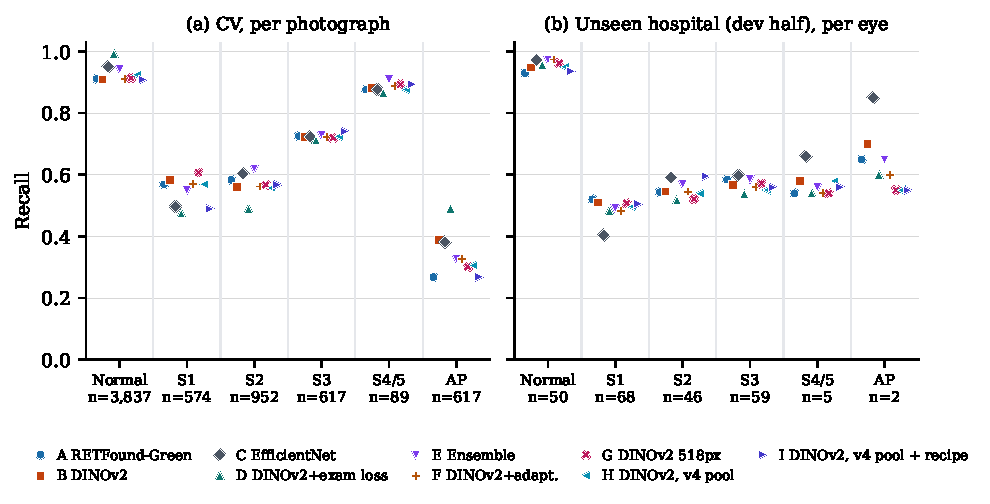
\includegraphics[width=\textwidth]{fig_stage_recall.pdf}
\caption{Recall per class, all transformer arms: (a) CV per photograph; (b) unseen hospital per eye. n below each class: photographs (a), eyes (b).}
\label{fig:stage}
\end{figure*}

\begin{figure*}[!t]
\centering
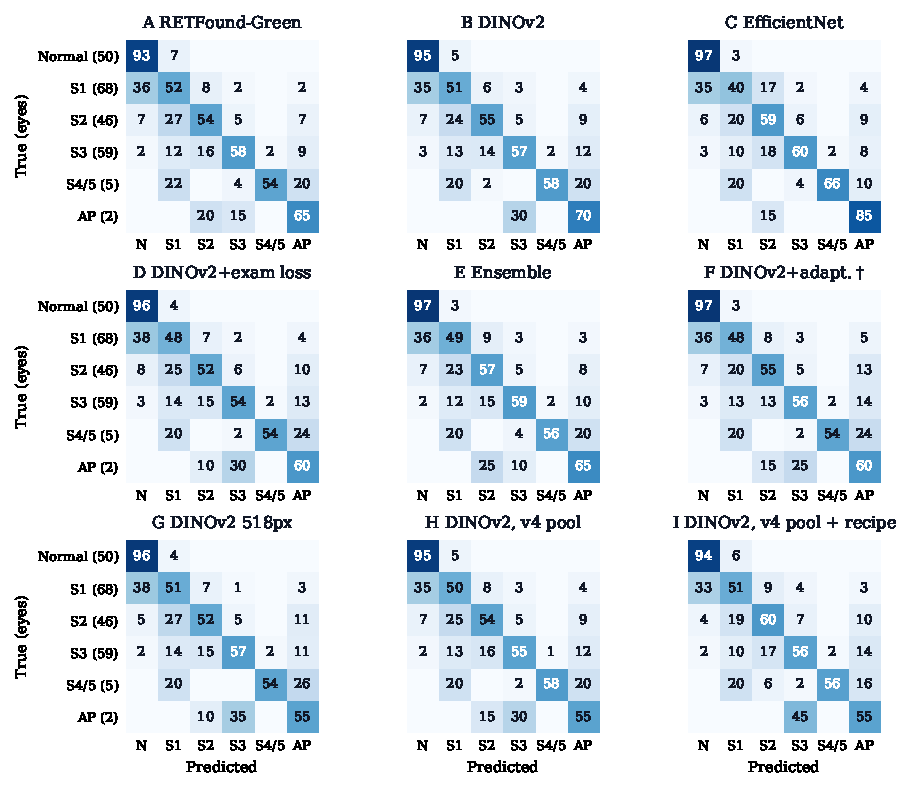
\includegraphics[width=0.8\textwidth]{fig_confusion_dev_eye.pdf}
\caption{Eye-level confusion matrices at the unseen hospital (development half), all arms. Cell: share of the true-class row in \%, averaged over each arm's \devLists{} models (diagonal = recall); blank = 0. True-class eye counts in parentheses.}
\label{fig:cm}
\end{figure*}

\subsection{Screening operating point and calibration}
Table~\ref{tab:operating} and Figs.~\ref{fig:roc}--\ref{fig:reliability} give the screening behaviour. B's operating point, the largest any-ROP threshold keeping cross-validation unit sensitivity at or above 0.90, sits at \BthrPct{} of the any-ROP score and gives cross-validation sensitivity \BcvSens{} at specificity \BcvSpec{}. Carried unchanged to the unseen hospital it catches \BdevSens{} of ROP eyes at specificity \BdevSpec{}, and \BdevSevereSens{} of eyes with stage~3 or worse; the eye-level any-ROP AUC there is \BdevAUC{}, so the model separates ROP from normal eyes well and it is the threshold that does not transfer. The eye-level ECE at the unseen hospital is \BdevECE{} as trained, and every cross-validation temperature made every arm more over-confident there, so the served application applies no temperature and labels the scores as uncalibrated. Neither the threshold nor the calibration transferred for any arm: both must be set at the site of use.

\begin{table*}[!t]
\caption{Operating point and calibration, per arm and seed. Threshold: the largest any-ROP score keeping CV unit-level sensitivity $\ge 0.90$; carried unchanged to the dev half. Severe: stage \nSevereFrom{} or worse, including AP-ROP. $T$: temperature fitted on CV out-of-fold unit vectors. ECE: ten bins, dev eyes, seeds pooled, as trained and after $T$.}
\label{tab:operating}
\centering\scriptsize\setlength{\tabcolsep}{2.4pt}
\begin{tabular}{@{}llc@{\hspace{5pt}}cccc@{\hspace{5pt}}cccc@{\hspace{5pt}}ccc@{}}
\toprule
 & & & \multicolumn{4}{c}{Any ROP vs normal} & \multicolumn{4}{c}{Severe (S3+) vs rest} & & \multicolumn{2}{c}{Dev-eye ECE}\\
\cmidrule(lr){4-7}\cmidrule(lr){8-11}\cmidrule(l){13-14}
Arm & Seed & Threshold & CV sens & CV spec & Dev sens & Dev spec & CV sens & CV spec & Dev sens & Dev spec & $T$ & as trained & with $T$\\
\midrule
A & 42 & 0.9884 & 0.900 & 0.999 & 0.650 & 1.000 & 0.952 & 0.652 & 0.924 & 0.659 & 0.840 & 0.152 & 0.205 \\
 & 1337 & 0.9887 & 0.900 & 0.996 & 0.670 & 1.000 & 0.955 & 0.651 & 0.933 & 0.640 & 0.853 &  &  \\
\textbf{B} & 42 & 0.9894 & 0.900 & 0.996 & 0.656 & 1.000 & 0.945 & 0.648 & 0.927 & 0.654 & 0.850 & 0.157 & 0.203 \\
 & 1337 & 0.9893 & 0.900 & 0.998 & 0.676 & 1.000 & 0.957 & 0.654 & 0.942 & 0.638 & 0.851 &  &  \\
C & 42 & 0.9850 & 0.900 & 0.991 & 0.680 & 1.000 & 0.948 & 0.646 & 0.894 & 0.613 & 0.917 & 0.183 & 0.208 \\
 & 1337 & 0.9805 & 0.900 & 0.993 & 0.671 & 1.000 & 0.942 & 0.645 & 0.918 & 0.633 & 0.935 &  &  \\
D & 42 & 0.9893 & 0.900 & 0.998 & 0.656 & 1.000 & 0.952 & 0.651 & 0.900 & 0.643 & 0.828 & 0.185 & 0.238 \\
 & 1337 & 0.9876 & 0.900 & 0.999 & 0.639 & 1.000 & 0.948 & 0.650 & 0.909 & 0.665 & 0.838 &  &  \\
E & 42 & 0.9866 & 0.900 & 1.000 & 0.650 & 1.000 & 0.945 & 0.650 & 0.912 & 0.654 & 0.747 & 0.135 & 0.214 \\
 & 1337 & 0.9848 & 0.900 & 0.998 & 0.662 & 1.000 & 0.941 & 0.647 & 0.918 & 0.643 & 0.762 &  &  \\
F$^\dagger$ & 42 & 0.9891 & 0.900 & 0.996 & 0.679 & 1.000 & 0.944 & 0.647 & 0.921 & 0.626 & 0.853 & 0.184 & 0.223 \\
 & 1337 & 0.9890 & 0.900 & 0.997 & 0.669 & 1.000 & 0.959 & 0.654 & 0.933 & 0.642 & 0.863 &  &  \\
G & 42 & 0.9882 & 0.900 & 0.996 & 0.643 & 1.000 & 0.949 & 0.649 & 0.921 & 0.665 & 0.854 & 0.174 & 0.210 \\
 & 1337 & 0.9897 & 0.900 & 0.996 & 0.667 & 1.000 & 0.955 & 0.651 & 0.939 & 0.646 & 0.868 &  &  \\
H & 42 & 0.9884 & 0.900 & 0.996 & 0.658 & 1.000 & 0.946 & 0.648 & 0.918 & 0.648 & 0.836 & 0.167 & 0.215 \\
 & 1337 & 0.9898 & 0.900 & 0.998 & 0.661 & 1.000 & 0.953 & 0.652 & 0.927 & 0.648 & 0.851 &  &  \\
I & 42 & 0.9812 & 0.900 & 0.998 & 0.676 & 1.000 & 0.937 & 0.646 & 0.912 & 0.626 & 0.620 & 0.061 & 0.196 \\
 & 1337 & 0.9816 & 0.900 & 0.998 & 0.680 & 1.000 & 0.938 & 0.646 & 0.918 & 0.623 & 0.631 &  &  \\
\bottomrule
\end{tabular}

\end{table*}

\begin{figure*}[!t]
\centering
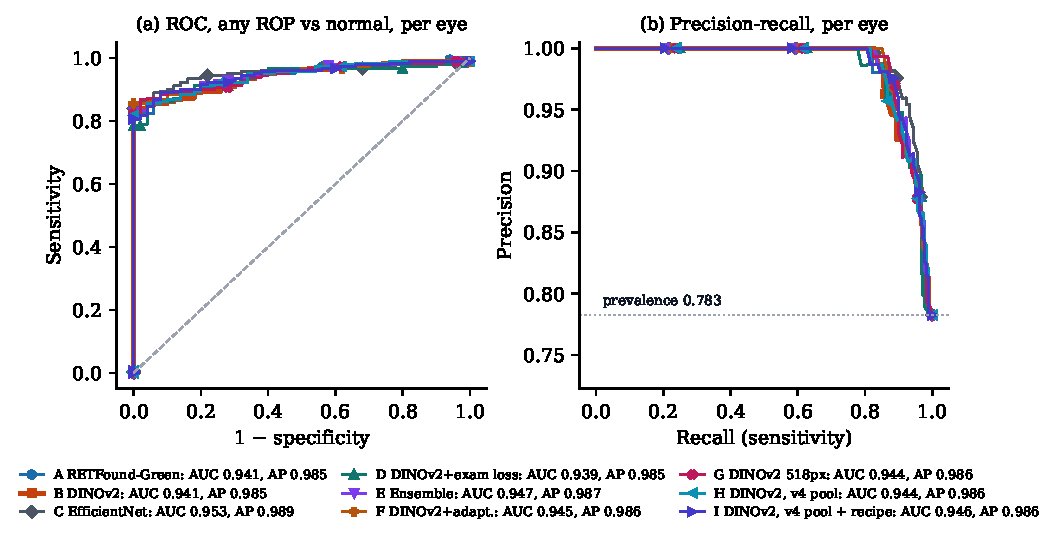
\includegraphics[width=\textwidth]{fig_roc_pr_dev_eye.pdf}
\caption{Any ROP vs normal per eye at the unseen hospital (development half), all arms: ROC and precision--recall, eye score averaged over each arm's \devLists{} models. Dotted: prevalence.}
\label{fig:roc}
\end{figure*}

\begin{figure*}[!t]
\centering
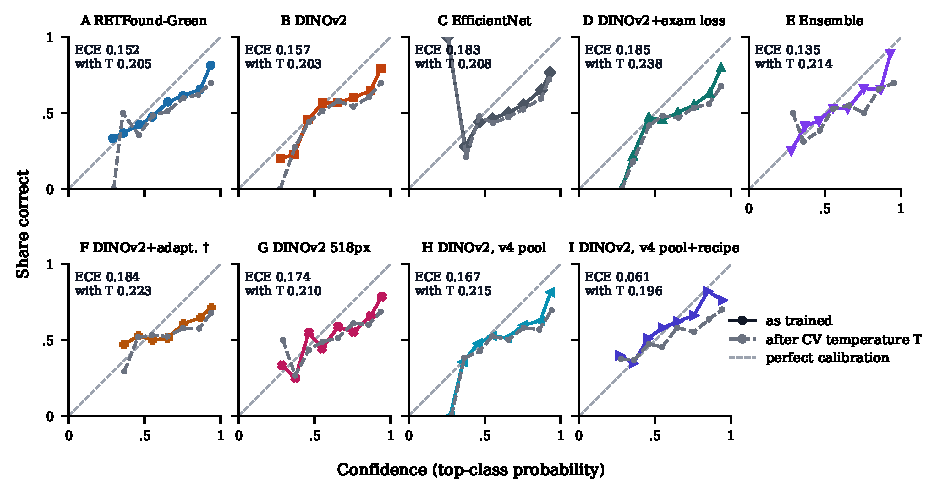
\includegraphics[width=\textwidth]{fig_reliability_dev_eye.pdf}
\caption{Reliability of the eye-level top-class probability at the unseen hospital, ten equal-width bins, seeds pooled: as trained (colour) and after each seed's CV temperature (grey). The temperature makes every arm more over-confident at the new site.}
\label{fig:reliability}
\end{figure*}

\subsection{Training at the label's unit}
Scored at each training cohort's own unit, arm D, whose loss sees an Ostrava examination session rather than a frame, scores QWK \DostravaQ{} on Ostrava examinations against \BostravaQ{} for B, the same encoder trained per photograph, and \CostravaQ{} for the CNN; on ROP-VL (\DropvlQ{} against \BropvlQ{}) and Shenzhen (\DshenzhenQ{} against \BshenzhenQ{}), whose labels are already per photograph, D is within noise of B, and at the unseen hospital it is slightly below B (\devDiffDB{} \devDiffDBci{}). The paired bootstrap over Ostrava sessions, reported in~\cite{nagpure2026}, puts the examination-level gain at about $+0.15$ QWK; it is post hoc, rests on 18 diseased infants and is confounded with Ostrava's share of training steps, so it is a hypothesis for a pre-registered follow-up. It is also the only change in the transformer generation with an effect larger than the confidence intervals.

\subsection{What the models look at}
Fig.~\ref{fig:gradcam} shows Grad-CAM~\cite{selvaraju2017} maps of the served ensemble for development-half photographs, with two measurements the application reports beside every map: the share of attention that fell outside the retinal field, on the camera's own surround, and how much of the frame holds half of the attention. We report these because an earlier cross-model comparison of raw off-retina attention turned out to measure letterboxing and the choice of objective rather than the model~\cite{nagpure2026}; the maps are shown as what moved the score, never as evidence of correctness.

\begin{figure*}[!t]
\centering
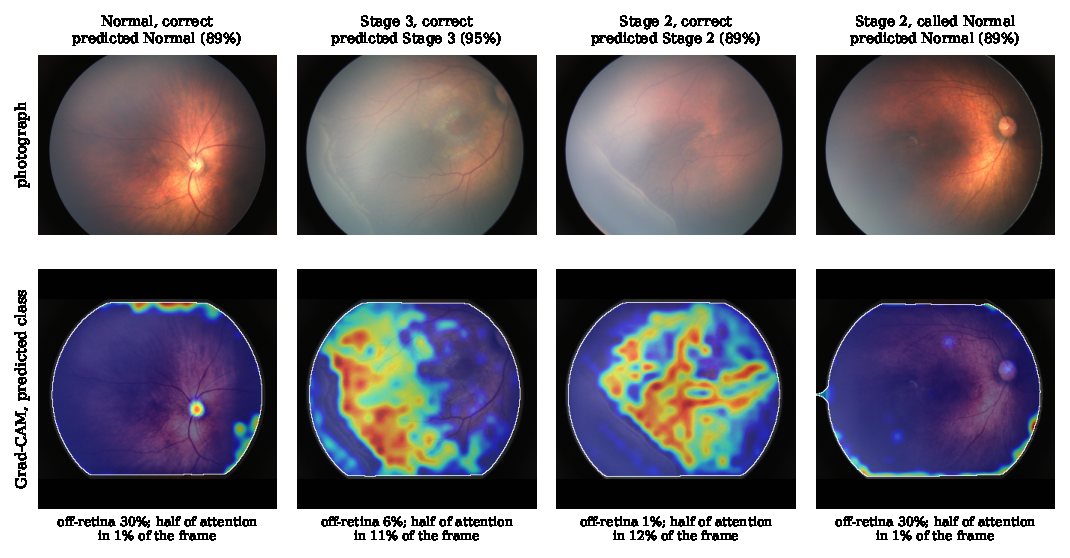
\includegraphics[width=\textwidth]{fig_gradcam.pdf}
\caption{Grad-CAM of the served ensemble (arm B, seed \seedA{}, five checkpoints) for development-half photographs: a correct normal, a correct stage 3, a correct stage 2, and a stage-2 photograph called normal. Maps are coloured inside the retinal field only; under each, the share of attention outside the retina and how much of the frame holds half of it.}
\label{fig:gradcam}
\end{figure*}

\subsection{Every generation at a glance}
Table~\ref{tab:best} lists the best model of each generation under its own protocol with the reason it is or is not comparable with B, and Fig.~\ref{fig:timeline} places them in time. The classical learners reach QWK \mateMLQ{} on their own photo-level test split; the CNNs 0.86--0.90 (photo-level, four classes) or \vTwoLockedEyeQ{} (patient-grouped, six classes, unseen hospital per eye, QWK5$_d$); the transformers \BdevQ{} (patient-grouped, six classes, unseen hospital per eye). Read down the table, the number rises and falls with the protocol far more than with the model family.

\begin{table*}[!t]
\caption{Every generation at a glance: the best model of each under its own protocol. Only one row is the project's selected model; every other row is listed with the reason its number cannot be read against it. Teammate rows: four classes, photo-level split, test n\,=\,\mateTest{} (\mateMLTest{} for rop\_ml); CI: 95\% Wilson~\cite{wilson1927}.}
\label{tab:best}
\centering\scriptsize\setlength{\tabcolsep}{4pt}
\begin{tabular}{@{}>{\raggedright\arraybackslash}p{1.55cm}>{\raggedright\arraybackslash}p{4.1cm}>{\raggedright\arraybackslash}p{3.0cm}>{\raggedright\arraybackslash}p{3.55cm}>{\raggedright\arraybackslash}p{4.9cm}@{}}
\toprule
Generation & Best model & Task; split; unit & Headline, own protocol & Comparable with B?\\
\midrule
v1, Jun 2026 & EfficientNet-B3, one model for ROP and DR & ROP yes/no; image-level split; photo & test acc.\ 0.733, ROP F1 0.706 & No: image-level split; other task (Table~\ref{tab:v1}) \\
Jun 2026 sweep & ResNet50 & ROP yes/no; Ostrava; photo & test AUC 0.927, QWK$_2$ 0.688 & No: device shortcut, AUC 0.911 from image size alone (Table~\ref{tab:sweep}) \\
v2, Aug 2026 & EfficientNetV2-S, structured head & 6 classes; patient-grouped 5-fold CV; photo / eye & CV QWK$_6$ 0.761; locked eye QWK5$_d$ 0.813 (seed 42) & No: own QWK definitions and checkpoint rule; re-scored as arm C (Table~\ref{tab:v2}) \\
v3/v4, Oct 2026 & \textbf{B: DINOv2 ViT-S/14, 5-fold ensemble (selected)} & 6 classes; protocol v2; photo / eye & CV QWK5 0.825 [0.737, 0.911]; unseen-hospital eye QWK5 0.756 [0.679, 0.821] & Reference (Table~\ref{tab:headline}); the served model \\
Teammate, Nov 2026 & rop\_ml: SVM (RBF) on 428 hand-made features & 4 classes; photo-level 80/20; photo & test acc.\ 0.585, QWK 0.547 & No: photo-level split (73\% of test photos share an infant with training); trained on 390 dev-half and 331 locked-half photos; four classes (Table~\ref{tab:mateml}) \\
 & rop\_cnn: resnest50d & 4 classes; photo-level 80/10/10; photo & test acc.\ 0.835, QWK 0.898 & As above (Table~\ref{tab:matecnn}) \\
 & rop\_foundation: RETFound-DINOv2 ViT-L/14 + LoRA, 3 seeds averaged & 4 classes; photo-level 80/10/10; photo & test acc.\ 0.844, QWK 0.900 & As above (Table~\ref{tab:matefm}) \\
 & \textbf{Best of the packages: 3 seeds + 4 CNNs averaged} & 4 classes; photo-level 80/10/10; photo & test acc.\ 0.860 [0.820, 0.896], QWK 0.908, AUC 0.972 & As above; selected on validation, 314 photos (Table~\ref{tab:matefm}) \\
\bottomrule
\end{tabular}

\end{table*}

\begin{figure*}[!t]
\centering
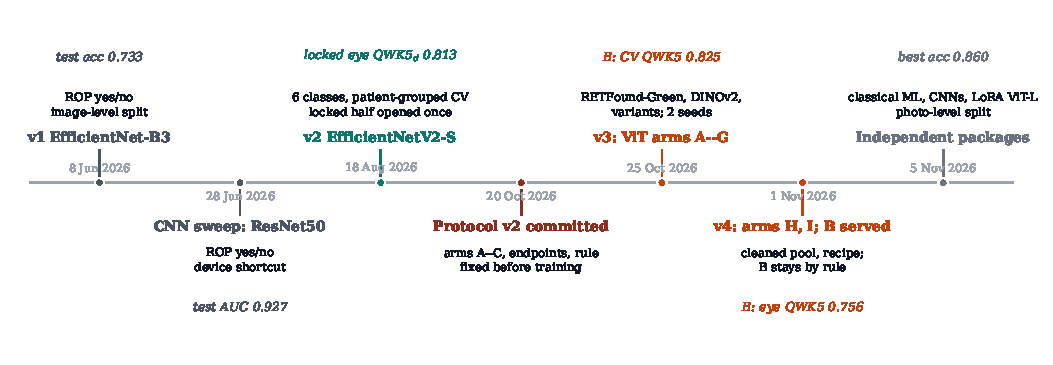
\includegraphics[width=\textwidth]{fig_timeline.pdf}
\caption{The development in time, with each generation's split type and its headline under its own protocol. Numbers across generations are not comparable (Table~\ref{tab:best}).}
\label{fig:timeline}
\end{figure*}

\subsection{The independent packages}\label{sec:mate}
Table~\ref{tab:matedata} shows the teammate's data against this project's splits: \mateMatched{} of \mateN{} photographs matched by file name; \mateDevTrain{} development-half and \mateLockedTrain{} locked-half photographs were used for training, so none of the three packages can ever be scored on this project's test halves; \mateLeakTest{} of their test photographs and \mateLeakVal{} of their validation photographs share an infant with their training set (\mateLeakMV{} of the Multi-View test photographs). Within the packages, the three seeds of the chosen foundation-model configuration reached test accuracy \mateFMlo{}--\mateFMhi{} (mean \mateFMmean{}, SD \mateFMsd{}), the attention-only adapters \mateFMbaseAcc{}, and four changes combined \mateFMcomboAcc{}; averaging the seeds gave \mateEnsAcc{} (QWK \mateEnsQ{}) and adding four CNNs the best number in the packages, \mateBestAcc{} \mateBestAccci{} (QWK \mateBestQ{}, AUC \mateBestAUC{}; Fig.~\ref{fig:teammate}). A frozen retina-pretrained ViT-L with \mateFMtrainable{}~M adapted weights thus ties fully fine-tuned CNNs, as arm A tied arm C; single-change recipe effects sit inside seed-to-seed spread; and averaging models is the only reliable gain. These are the same three conclusions the pre-registered generation reached, at a higher absolute level set by the split.

\begin{table*}[!t]
\caption{Teammate packages: their photo-level split against this project's splits, by file name. ``Elsewhere'': renamed copies not matched. Last column: validation/test photographs whose infant also has photographs in their training set.}
\label{tab:matedata}
\centering\scriptsize\setlength{\tabcolsep}{4pt}
\begin{tabular}{@{}lr@{\hspace{6pt}}rrrr@{\hspace{6pt}}rrrr@{\hspace{6pt}}c@{}}
\toprule
 & & \multicolumn{4}{c}{Their classes} & \multicolumn{4}{c}{Where the photographs sit in this project} & Same infant\\
\cmidrule(lr){3-6}\cmidrule(lr){7-10}
Their split & Photos & N & S1 & S2 & S3 & CV pool & Dev half & Locked half & Elsewhere & as their training\\
\midrule
Train & 2{,}512 & 687 & 515 & 651 & 659 & 1{,}647 & 390 & 331 & 144 & -- \\
Val & 314 & 86 & 65 & 81 & 82 & 208 & 48 & 39 & 19 & 214 / 295 \\
Test & 315 & 86 & 64 & 82 & 83 & 213 & 50 & 38 & 14 & 221 / 301 \\
\bottomrule
\end{tabular}

\end{table*}

\begin{figure}[!t]
\centering
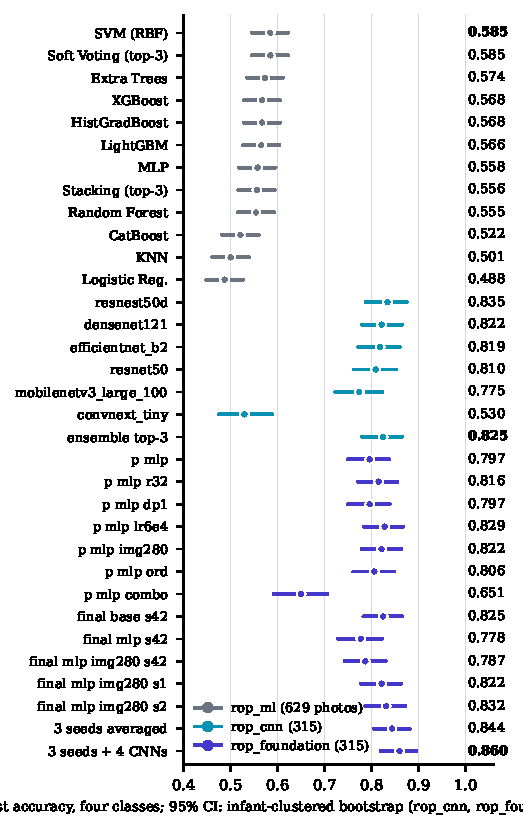
\includegraphics[width=\columnwidth]{fig_teammate.pdf}
\caption{Independent packages: four-class test accuracy of every model with 95\% Wilson CI, one colour per package. Dotted: chance. Not comparable with Figs.~\ref{fig:selection}--\ref{fig:dev}.}
\label{fig:teammate}
\end{figure}

\subsection{The served system}
The selected ensemble is served in a single-page web application (Fig.~\ref{fig:webapp}) that requires the operator to declare the patient population before any model runs, gates ungradable photographs, reports the screening verdict against the fixed operating point with the measured sensitivities beside it, the six-class stage as a research output, the Grad-CAM with its two measurements, a whole-eye mode applying the most-severe-photograph rule, and a PDF report. Beside the served stage it shows the stage of the teammate's three-seed RETFound-DINOv2 ensemble with an agree/disagree mark; that model never decides anything, and the page states its provenance. A seen-photo guard hashes every upload against the \stageLabelled{} photographs of the project's data and flags any that a model trained or was tested on, because a demonstration on such a photograph is not a test of either model.

\begin{figure*}[!t]
\centering
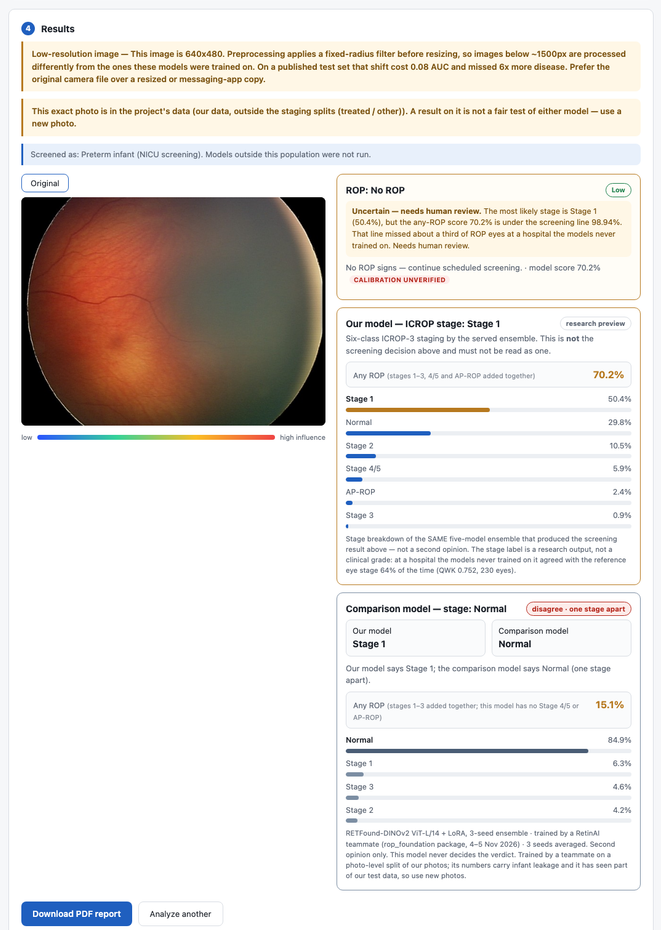
\includegraphics[width=0.92\textwidth]{fig_webapp.png}
\caption{The served application on a development-half photograph: verdict against the fixed operating point, the served model's stage, the comparison model's stage with the agreement mark, and the seen-photo notice. Research prototype; not a medical device.}
\label{fig:webapp}
\end{figure*}

\section{Discussion}\label{sec:discussion}
This development started where many ROP studies start and ended where many now end, and the lesson of the path is that the measurement moved the number more than the model did. Three methodological choices decided the headline at every stage. The \emph{split}: by photograph, classical learners reach QWK \mateMLQ{} and CNNs 0.9 on this corpus (Section~\ref{sec:mate}); by infant, the same CNN family scores \vTwoLockedEyeQ{} at an unseen hospital. The \emph{unit}: the same predictions score \vTwoLockedImgQ{} per photograph and \vTwoLockedEyeQ{} per eye, because labels given per eye or per session are inherited by frames that do not show the finding. The \emph{site}: a screening head with 0.97 AUC at home flagged every photograph at the first unseen hospital, and no operating point or temperature fitted in cross-validation transferred for any of nine transformer arms. Against these, the architecture choices of three generations moved nothing that survived a change of random seed: ordinal versus flat heads, five CNN backbones, retinal versus natural pre-training, resolution, ensembling, decoding, unsupervised adaptation, a cleaned pool and a stronger recipe all lie inside one arm's confidence interval. The one exception, training at the unit the label describes (arm D), moved the Ostrava examination-level result by about 0.15 and nothing elsewhere, because elsewhere the labels are already per photograph.

The pre-training null agrees with ROP-Bench~\cite{luo2026} and Mahboob et al.~\cite{mahboob2025}, extended here to multi-class staging with the architecture confound removed, and the teammate's package reproduces it with a frozen ViT-L and low-rank adapters. The adapter result is itself useful: \mateFMtrainable{}~M trainable weights on a frozen retina-pretrained backbone matched fully fine-tuned CNNs, so a site wishing to adapt a foundation model needs to train and store very little.

Our numbers are unremarkable next to the published state of the art, and we think that is the honest position. Against inter-expert kappa \humanInterKappa{} and intra-expert \humanIntraKappa{} on this task~\cite{gschliesser2015}, reported model agreements above 0.95 warrant scrutiny rather than celebration; our own unweighted eye-level kappa at the unseen hospital (\BdevKappaU{}) exceeds the inter-expert value, with the caveat that these are different quantities on different images against a single institution's coding practice. The errors that remain, normal/stage 1 and stage 1/stage 2, are where experts disagree most, and a model trained on three institutions' reading of the stage-1 boundary cannot agree with a fourth's reading better than experts agree with each other. Eye-level training labels and clinician re-grading of the photographs on which several independent models disagree with the label are the inputs most likely to raise the ceiling; another backbone is not.

Clinically, the findings argue for three practices: report the eye, not the photograph, with the driving photograph shown; set the screening threshold and the calibration at the site of use; and show the operator the model's provenance and the limits of its evidence, which the served application does by stating its measured sensitivities, labelling its scores uncalibrated, and declining photographs it has seen.

This study has several limitations. First, labels were not re-graded and two cohorts label per examination, so some training labels describe frames that do not show the finding. Second, the severe classes have five and two eyes at the unseen hospital and are not evaluated there; AP-ROP in cross-validation is dominated by one infant. Third, the unseen hospital's development half was used for design decisions in the CNN generation and has now been examined for nine transformer arms, so its numbers are descriptive and any difference there is one look of many; the locked half, which carries the pre-registered primary endpoint, remains unscored for the transformers. Fourth, two seeds per arm bound seed variability only coarsely. Fifth, the independent packages were trained outside the protocol on a photo-level split that overlaps the test halves; they are reported for what they show about splits, not as results. Sixth, the corpus carries no zone or plus-disease annotation, so the criteria on which treatment decisions rest are outside its scope. Seventh, the classical-learner stage was run on four classes with the independent package's features; a classical baseline under the full protocol was not trained.

\section{Conclusion}
Over three generations on an audited four-hospital corpus, the methodological choices, the split, the label unit and the site of the threshold, decided the reported numbers, and the models did not. The selected five-fold DINOv2 ensemble reaches eye-level QWK \BdevQ{} and any-ROP AUC \BdevAUC{} at a hospital it never saw; retina-pretrained, CNN and adapter-based alternatives tie it; a photo-level split lifts the same families to accuracies that mean nothing outside the split. Training at the unit the label describes is the one change with an effect to pursue. We release every number with the file it comes from, and we suggest that ICROP staging studies state the unit their labels describe, split by infant, score at the eye, validate at an unseen hospital before a threshold is deployed, and show the reader where each number came from.

\section*{Compliance with Ethical Standards}
This retrospective study used only publicly released, de-identified datasets under their licences (Ostrava/RIDIRP, CC0; ROP-VL and Shenzhen, CC BY 4.0; Multi-View ROP, CC BY-NC 4.0); no new data were collected and no ethical approval was required. RETFound-Green's and RETFound-DINOv2's weights are used under their non-commercial licences. The system is research software and not a medical device. No funding was received; the authors declare no conflicts of interest.

\section*{Data and Code Availability}
The four cohorts are public at the sources cited. The protocol, its amendments, the result files, the scripts that generate every figure, table and number of this paper, and the served application are at \FILL{repository URL}. No file of the locked half was read by any script of this paper.

\section*{Acknowledgments}
We thank the releasing institutions and Kaggle for the free GPU time on which every model was trained, and \FILL{teammate's name} for the independent packages of Sections~\ref{sec:ml}--\ref{sec:vit}. \FILL{venue-specific AI disclosure, e.g.: Claude (Anthropic) was used to draft and edit code and text in all sections under the authors' direction; the authors verified every number against the committed result files and take full responsibility for the content.}

\begin{thebibliography}{99}
\bibitem{blencowe2013} H.~Blencowe, J.~E.~Lawn, T.~Vazquez, A.~Fielder, and C.~Gilbert, ``Preterm-associated visual impairment and estimates of retinopathy of prematurity at regional and global levels for 2010,'' \emph{Pediatr. Res.}, vol.~74, suppl.~1, pp.~35--49, 2013.
\bibitem{icrop3} M.~F.~Chiang, G.~E.~Quinn, A.~R.~Fielder, \emph{et al.}, ``International classification of retinopathy of prematurity, third edition,'' \emph{Ophthalmology}, vol.~128, no.~10, pp.~e51--e68, 2021.
\bibitem{etrop2003} Early Treatment for Retinopathy of Prematurity Cooperative Group, ``Revised indications for the treatment of retinopathy of prematurity: results of the Early Treatment for Retinopathy of Prematurity randomized trial,'' \emph{Arch. Ophthalmol.}, vol.~121, no.~12, pp.~1684--1694, 2003.
\bibitem{vahid2026} M.~Vahidmoghadam, P.~Ghorbani, M.~J.~Ahmadi, \emph{et al.}, ``Automated diagnosis of plus form and early stages of ROP using deep learning models,'' \emph{Sci. Rep.}, vol.~16, art.~7234, 2026.
\bibitem{gschliesser2015} A.~Gschlie\ss{}er, E.~Stifter, T.~Neumayer, \emph{et al.}, ``Inter-expert and intra-expert agreement on the diagnosis and treatment of retinopathy of prematurity,'' \emph{Am. J. Ophthalmol.}, vol.~160, no.~3, pp.~553--560, 2015.
\bibitem{campbell2016} J.~P.~Campbell, S.~N.~Ryan, E.~Lore, \emph{et al.}, ``Diagnostic discrepancies in retinopathy of prematurity classification,'' \emph{Ophthalmology}, vol.~123, no.~8, pp.~1795--1801, 2016.
\bibitem{nagpure2026} P.~Nagpure, R.~Bait, P.~Rangnekar, Y.~Shengale, and A.~Kumar, ``What the label unit hides: an audited multi-hospital benchmark for ICROP retinopathy of prematurity staging,'' \FILL{preprint venue, DOI, 2026}.
\bibitem{timkovic2024} J.~Timkovi\v{c}, \emph{et al.}, ``Retinal image dataset of infants and retinopathy of prematurity,'' \emph{Sci. Data}, vol.~11, art.~814, 2024.
\bibitem{zhao2024} J.~Zhao, \emph{et al.}, ``\FILL{confirm title}: a fundus image dataset for retinopathy of prematurity,'' \emph{Sci. Data}, vol.~11, 2024, figshare doi:10.6084/m9.figshare.25514449. \FILL{confirm authors, title and article number}
\bibitem{ropvl2026} \FILL{author list}, ``ROP-VL: \FILL{confirm title},'' \emph{Sci. Data}, 2026, doi:10.1038/s41597-026-07901-0; data doi:10.6084/m9.figshare.30143461.
\bibitem{multiview2026} L.~Liao, \emph{et al.}, ``Multi-View ROP dataset,'' Hugging Face dataset \texttt{lijuanliao/ROP-DATASET}, 2026, CC BY-NC 4.0. \FILL{confirm authors and any accompanying publication}
\bibitem{wang2026} \FILL{author list}, ``VEA-Net: vascular enhancement attention network for multi-task retinopathy of prematurity classification,'' \emph{Front. Cell Dev. Biol.}, 2026. \FILL{confirm volume and article number}
\bibitem{peng2021} Y.~Peng, W.~Zhu, Z.~Chen, \emph{et al.}, ``Automatic staging for retinopathy of prematurity with deep feature fusion and ordinal classification strategy,'' \emph{IEEE Trans. Med. Imaging}, vol.~40, no.~7, pp.~1750--1762, 2021.
\bibitem{brown2018} J.~M.~Brown, J.~P.~Campbell, A.~Beers, \emph{et al.}, ``Automated diagnosis of plus disease in retinopathy of prematurity using deep convolutional neural networks,'' \emph{JAMA Ophthalmol.}, vol.~136, no.~7, pp.~803--810, 2018.
\bibitem{derks2025} \FILL{author list} and J.~P.~Campbell, ``External validation of the i-ROP deep learning system,'' \emph{J. AAPOS}, 2025. \FILL{confirm title, volume, pages}
\bibitem{wang2021} J.~Wang, J.~Ji, M.~Zhang, \emph{et al.}, ``Automated explainable multidimensional deep learning platform of retinal images for retinopathy of prematurity screening,'' \emph{JAMA Netw. Open}, vol.~4, no.~5, e218758, 2021.
\bibitem{lan2026} W.-H.~Lan, C.-L.~Tsai, and W.-C.~Wu, ``Optimizing field-of-view for type-1 retinopathy of prematurity via multiple instance learning,'' \emph{Transl. Vis. Sci. Technol.}, vol.~15, no.~8, art.~13, 2026, doi:10.1167/tvst.15.8.13.
\bibitem{zhou2023} Y.~Zhou, M.~A.~Chia, S.~K.~Wagner, \emph{et al.}, ``A foundation model for generalizable disease detection from retinal images,'' \emph{Nature}, vol.~622, pp.~156--163, 2023.
\bibitem{engelmann2025} J.~Engelmann, \emph{et al.}, ``RETFound-Green: a green retinal foundation model,'' \emph{Nat. Commun.}, 2025. \FILL{confirm title, volume, article number}
\bibitem{luo2026} Luo, Guo, Chen, Liang, and Lin, ``ROP-Bench: a benchmark of foundation models for retinopathy of prematurity,'' Zenodo record 20721027, 2026. \FILL{confirm author list and title}
\bibitem{oquab2024} M.~Oquab, T.~Darcet, T.~Moutakanni, \emph{et al.}, ``DINOv2: learning robust visual features without supervision,'' \emph{Trans. Mach. Learn. Res.}, 2024.
\bibitem{mahboob2025} Z.~Mahboob, A.~O.~Ahsan, and M.~Wilms, ``Using an adult retinal image analysis foundation model for retinopathy of prematurity staging: are there benefits?'' in \emph{Proc. SPIE Medical Imaging 2025: Computer-Aided Diagnosis}, 2025, doi:10.1117/12.3047303. \FILL{confirm volume and paper number}
\bibitem{chen2025} \FILL{author list}, ``SABPI-Net \FILL{full title},'' in \emph{Proc. MICCAI}, 2025.
\bibitem{zhao2026} Zhao and Li, ``DeepAdapter: self-supervised pre-training and domain adaptation for retinopathy of prematurity screening,'' \emph{Br. J. Ophthalmol.}, 2026, doi:10.1136/bjo-2025-328559. \FILL{confirm title and authors}
\bibitem{ojala2002} T.~Ojala, M.~Pietik\"ainen, and T.~M\"aenp\"a\"a, ``Multiresolution gray-scale and rotation invariant texture classification with local binary patterns,'' \emph{IEEE Trans. Pattern Anal. Mach. Intell.}, vol.~24, no.~7, pp.~971--987, 2002.
\bibitem{haralick1973} R.~M.~Haralick, K.~Shanmugam, and I.~Dinstein, ``Textural features for image classification,'' \emph{IEEE Trans. Syst., Man, Cybern.}, vol.~SMC-3, no.~6, pp.~610--621, 1973.
\bibitem{dalal2005} N.~Dalal and B.~Triggs, ``Histograms of oriented gradients for human detection,'' in \emph{Proc. IEEE CVPR}, 2005, pp.~886--893.
\bibitem{frangi1998} A.~F.~Frangi, W.~J.~Niessen, K.~L.~Vincken, and M.~A.~Viergever, ``Multiscale vessel enhancement filtering,'' in \emph{Proc. MICCAI}, LNCS vol.~1496, 1998, pp.~130--137.
\bibitem{geirhos2020} R.~Geirhos, J.-H.~Jacobsen, C.~Michaelis, \emph{et al.}, ``Shortcut learning in deep neural networks,'' \emph{Nat. Mach. Intell.}, vol.~2, pp.~665--673, 2020.
\bibitem{degrave2021} A.~J.~DeGrave, J.~D.~Janizek, and S.-I.~Lee, ``AI for radiographic COVID-19 detection selects shortcuts over signal,'' \emph{Nat. Mach. Intell.}, vol.~3, pp.~610--619, 2021.
\bibitem{oakden2020} L.~Oakden-Rayner, J.~Dunnmon, G.~Carneiro, and C.~R\'e, ``Hidden stratification causes clinically meaningful failures in machine learning for medical imaging,'' in \emph{Proc. ACM CHIL}, 2020, pp.~151--159.
\bibitem{tejani2024} A.~S.~Tejani, M.~E.~Klontzas, A.~A.~Gatti, \emph{et al.}, ``Checklist for Artificial Intelligence in Medical Imaging (CLAIM): 2024 update,'' \emph{Radiol. Artif. Intell.}, vol.~6, no.~4, e240300, 2024.
\bibitem{collins2024} G.~S.~Collins, K.~G.~M.~Moons, P.~Dhiman, \emph{et al.}, ``TRIPOD+AI statement: updated guidance for reporting clinical prediction models that use regression or machine learning methods,'' \emph{BMJ}, vol.~385, e078378, 2024.
\bibitem{zuiderveld1994} K.~Zuiderveld, ``Contrast limited adaptive histogram equalization,'' in \emph{Graphics Gems IV}, P.~S.~Heckbert, Ed. Academic Press, 1994, pp.~474--485.
\bibitem{cortes1995} C.~Cortes and V.~Vapnik, ``Support-vector networks,'' \emph{Mach. Learn.}, vol.~20, pp.~273--297, 1995.
\bibitem{breiman2001} L.~Breiman, ``Random forests,'' \emph{Mach. Learn.}, vol.~45, pp.~5--32, 2001.
\bibitem{chen2016} T.~Chen and C.~Guestrin, ``XGBoost: a scalable tree boosting system,'' in \emph{Proc. ACM SIGKDD}, 2016, pp.~785--794.
\bibitem{ke2017} G.~Ke, Q.~Meng, T.~Finley, \emph{et al.}, ``LightGBM: a highly efficient gradient boosting decision tree,'' in \emph{Proc. NeurIPS}, 2017.
\bibitem{prokhorenkova2018} L.~Prokhorenkova, G.~Gusev, A.~Vorobev, A.~V.~Dorogush, and A.~Gulin, ``CatBoost: unbiased boosting with categorical features,'' in \emph{Proc. NeurIPS}, 2018.
\bibitem{tan2019} M.~Tan and Q.~V.~Le, ``EfficientNet: rethinking model scaling for convolutional neural networks,'' in \emph{Proc. ICML}, 2019, pp.~6105--6114.
\bibitem{tan2021} M.~Tan and Q.~V.~Le, ``EfficientNetV2: smaller models and faster training,'' in \emph{Proc. ICML}, 2021, pp.~10096--10106.
\bibitem{howard2019} A.~Howard, M.~Sandler, G.~Chu, \emph{et al.}, ``Searching for MobileNetV3,'' in \emph{Proc. IEEE/CVF ICCV}, 2019, pp.~1314--1324.
\bibitem{he2016} K.~He, X.~Zhang, S.~Ren, and J.~Sun, ``Deep residual learning for image recognition,'' in \emph{Proc. IEEE CVPR}, 2016, pp.~770--778.
\bibitem{huang2017} G.~Huang, Z.~Liu, L.~van der Maaten, and K.~Q.~Weinberger, ``Densely connected convolutional networks,'' in \emph{Proc. IEEE CVPR}, 2017, pp.~4700--4708.
\bibitem{chen2021} J.~S.~Chen, A.~S.~Coyner, S.~Ostmo, \emph{et al.}, ``Deep learning for the diagnosis of stage in retinopathy of prematurity: accuracy and generalizability across populations and cameras,'' \emph{Ophthalmol. Retina}, vol.~5, no.~10, pp.~1027--1035, 2021.
\bibitem{corn2023} X.~Shi, W.~Cao, and S.~Raschka, ``Deep neural networks for rank-consistent ordinal regression based on conditional probabilities,'' \emph{Pattern Anal. Appl.}, vol.~26, pp.~941--955, 2023.
\bibitem{ganin2016} Y.~Ganin, E.~Ustinova, H.~Ajakan, \emph{et al.}, ``Domain-adversarial training of neural networks,'' \emph{J. Mach. Learn. Res.}, vol.~17, no.~59, pp.~1--35, 2016.
\bibitem{liu2022} Z.~Liu, H.~Mao, C.-Y.~Wu, C.~Feichtenhofer, T.~Darrell, and S.~Xie, ``A ConvNet for the 2020s,'' in \emph{Proc. IEEE/CVF CVPR}, 2022, pp.~11976--11986.
\bibitem{zhang2022} H.~Zhang, C.~Wu, Z.~Zhang, \emph{et al.}, ``ResNeSt: split-attention networks,'' in \emph{Proc. IEEE/CVF CVPR Workshops}, 2022, pp.~2736--2746.
\bibitem{wightman2019} R.~Wightman, ``PyTorch image models,'' GitHub repository, 2019, doi:10.5281/zenodo.4414861.
\bibitem{loshchilov2019} I.~Loshchilov and F.~Hutter, ``Decoupled weight decay regularization,'' in \emph{Proc. ICLR}, 2019.
\bibitem{dosovitskiy2021} A.~Dosovitskiy, L.~Beyer, A.~Kolesnikov, \emph{et al.}, ``An image is worth 16$\times$16 words: transformers for image recognition at scale,'' in \emph{Proc. ICLR}, 2021.
\bibitem{cui2019} Y.~Cui, M.~Jia, T.-Y.~Lin, Y.~Song, and S.~Belongie, ``Class-balanced loss based on effective number of samples,'' in \emph{Proc. IEEE/CVF CVPR}, 2019, pp.~9268--9277.
\bibitem{french2018} G.~French, M.~Mackiewicz, and M.~Fisher, ``Self-ensembling for visual domain adaptation,'' in \emph{Proc. ICLR}, 2018.
\bibitem{cohen1968} J.~Cohen, ``Weighted kappa: nominal scale agreement with provision for scaled disagreement or partial credit,'' \emph{Psychol. Bull.}, vol.~70, no.~4, pp.~213--220, 1968.
\bibitem{guo2017} C.~Guo, G.~Pleiss, Y.~Sun, and K.~Q.~Weinberger, ``On calibration of modern neural networks,'' in \emph{Proc. ICML}, 2017, pp.~1321--1330.
\bibitem{hu2022} E.~J.~Hu, Y.~Shen, P.~Wallis, \emph{et al.}, ``LoRA: low-rank adaptation of large language models,'' in \emph{Proc. ICLR}, 2022.
\bibitem{selvaraju2017} R.~R.~Selvaraju, M.~Cogswell, A.~Das, R.~Vedantam, D.~Parikh, and D.~Batra, ``Grad-CAM: visual explanations from deep networks via gradient-based localization,'' in \emph{Proc. IEEE ICCV}, 2017, pp.~618--626.
\bibitem{wilson1927} E.~B.~Wilson, ``Probable inference, the law of succession, and statistical inference,'' \emph{J. Am. Stat. Assoc.}, vol.~22, no.~158, pp.~209--212, 1927.
\end{thebibliography}
\end{document}
